\documentclass[11pt, letterpaper]{article}

% Fonts and Encoding
\usepackage[utf8]{inputenc}
\usepackage[T1]{fontenc}
\usepackage{lmodern} % High-quality Latin Modern vector font

% Math and Symbols
\usepackage{amsmath, amssymb, amsthm, amsfonts, mathrsfs, mathtools}

% Layout and Geometry
\usepackage{geometry}
\geometry{letterpaper, margin=1in}
\setlength{\parindent}{0pt}
\setlength{\parskip}{0.6em}

% Formatting and Graphics
\usepackage{graphicx, xcolor, enumitem, booktabs, array, tabularx}

% TikZ for Illustrations
\usepackage{tikz}
\usetikzlibrary{arrows.meta, positioning, shapes.geometric, calc, backgrounds, matrix}

% Clickable Links and TOC
\usepackage{hyperref}
\hypersetup{
    colorlinks=true,
    linkcolor=blue,
    filecolor=magenta,      
    urlcolor=cyan,
    pdftitle={Advanced Mathematics Topic},
}

% Theorem Environments
\newtheorem{theorem}{Theorem}[section]
\newtheorem{lemma}[theorem]{Lemma}
\newtheorem{proposition}[theorem]{Proposition}
\newtheorem{corollary}[theorem]{Corollary}
\theoremstyle{definition}
\newtheorem{definition}{Definition}[section]
\newtheorem{axiom}{Axiom}[section]
\newtheorem{example}{Example}[section]
\theoremstyle{remark}
\newtheorem{remark}{Remark}[section]

% Custom Commands (Enforced standard notation)
\newcommand{\R}{\mathbb{R}}
\newcommand{\N}{\mathbb{N}}
\newcommand{\Z}{\mathbb{Z}}
\newcommand{\Q}{\mathbb{Q}}
\newcommand{\E}{\mathbb{E}}
\newcommand{\Prob}{\mathbb{P}}
\newcommand{\F}{\mathcal{F}}

\title{\textbf{Foundations of Multivariate Probability Distributions: Measure-Theoretic Intersections, Random Vectors, and Quantitative Modeling}}
\author{Tashfeen Omran}
\date{\today}

\begin{document}

\maketitle
\tableofcontents
\newpage

% ==============================================================================
% PART 1: COMPREHENSIVE INTRODUCTION, CONTEXT, AND PREREQUISITES
% ==============================================================================
\section{Comprehensive Introduction, Context, and Prerequisites}

\subsection{Core Concepts and Axioms}

In univariate probability theory, an experimenter observes a single numerical characteristic of a random phenomenon, modeled as a measurable function $Y : \Omega \to \R$ defined on an underlying probability space $(\Omega, \F, \Prob)$. However, both theoretical mathematics and empirical science demand the simultaneous analysis of multiple interacting quantities. Whether one is observing the joint outcome of a sequence of card draws, the litter size and survival count of biological organisms, the coupled height and weight of an individual, or an $n$-dimensional sample $(Y_1, Y_2, \dots, Y_n)$ drawn from a population, the fundamental mathematical object of interest is the \textbf{intersection of events} and its functional generalization: the \textbf{random vector}.

\begin{definition}[Probability Space and Set-Theoretic Intersection]
Let $\Omega$ be a non-empty set called the \emph{sample space}, whose elements $\omega \in \Omega$ are called \emph{sample points} or elementary outcomes. Let $\F \subseteq \mathcal{P}(\Omega)$ be a $\sigma$-algebra of subsets of $\Omega$ (called \emph{events}), and let $\Prob : \F \to [0, 1]$ be a countably additive probability measure satisfying $\Prob(\Omega) = 1$. Given a finite collection of events $A_1, A_2, \dots, A_n \in \F$, their simultaneous occurrence is represented by the set-theoretic intersection:
\[
\bigcap_{i=1}^{n} A_i = A_1 \cap A_2 \cap \cdots \cap A_n = \{\omega \in \Omega : \omega \in A_i \text{ for all } i \in \{1, 2, \dots, n\}\}.
\]
Because $\F$ is closed under countable unions and complementation, De Morgan's Laws guarantee that $\bigcap_{i=1}^{n} A_i = \left(\bigcup_{i=1}^{n} A_i^c\right)^c \in \F$, ensuring that the probability of the intersection $\Prob\left(\bigcap_{i=1}^{n} A_i\right)$ is always well-defined.
\end{definition}

\begin{definition}[Random Vector and Multivariate Measurability]
Let $(\Omega, \F, \Prob)$ be a probability space, and let $(\R^n, \mathcal{B}(\R^n))$ be the $n$-dimensional Euclidean space equipped with the Borel $\sigma$-algebra $\mathcal{B}(\R^n) = \mathcal{B}(\R) \otimes \mathcal{B}(\R) \otimes \cdots \otimes \mathcal{B}(\R)$, generated by $n$-dimensional open (or half-open) rectangles. An $n$-dimensional \emph{random vector} is a function $\mathbf{Y} = (Y_1, Y_2, \dots, Y_n) : \Omega \to \R^n$ defined componentwise by
\[
\mathbf{Y}(\omega) = \bigl(Y_1(\omega), Y_2(\omega), \dots, Y_n(\omega)\bigr) \quad \text{for all } \omega \in \Omega,
\]
such that for every Borel set $B \in \mathcal{B}(\R^n)$, the preimage (inverse image) lies in the event space:
\[
\mathbf{Y}^{-1}(B) = \{\omega \in \Omega : \mathbf{Y}(\omega) \in B\} \in \F.
\]
When $n = 2$, the pair $(Y_1, Y_2)$ is called a \emph{bivariate random vector}, and its induced probability law is called a \emph{bivariate probability distribution}. For general $n \ge 2$, it is called a \emph{multivariate probability distribution}.
\end{definition}

\begin{definition}[Induced Probability Measure (Pushforward Distribution)]
Given an $n$-dimensional random vector $\mathbf{Y} : \Omega \to \R^n$, the \emph{induced probability measure} (or \emph{pushforward measure}) $\Prob_{\mathbf{Y}} : \mathcal{B}(\R^n) \to [0, 1]$ is defined for every $B \in \mathcal{B}(\R^n)$ by
\[
\Prob_{\mathbf{Y}}(B) = \Prob\bigl(\mathbf{Y}^{-1}(B)\bigr) = \Prob\bigl(\{\omega \in \Omega : (Y_1(\omega), Y_2(\omega), \dots, Y_n(\omega)) \in B\}\bigr).
\]
In particular, if $B = B_1 \times B_2 \times \cdots \times B_n$ is a Cartesian product of univariate Borel sets $B_i \in \mathcal{B}(\R)$, then the preimage of the Cartesian product is precisely the intersection of the component preimages:
\[
\mathbf{Y}^{-1}(B_1 \times B_2 \times \cdots \times B_n) = \bigcap_{i=1}^{n} Y_i^{-1}(B_i) = \bigcap_{i=1}^{n} \{\omega \in \Omega : Y_i(\omega) \in B_i\}.
\]
In standard statistical notation, the comma inside a probability statement is syntactic shorthand for set intersection:
\[
\Prob(Y_1 = y_1, Y_2 = y_2, \dots, Y_n = y_n) \equiv \Prob\left(\bigcap_{i=1}^{n} \{\omega \in \Omega : Y_i(\omega) = y_i\}\right).
\]
\end{definition}

\begin{definition}[Discrete Bivariate and Multivariate Probability Mass Function]
Let $(Y_1, Y_2)$ be a discrete bivariate random vector taking values in a countable support set $\mathcal{S} \subseteq \R^2$. The \emph{bivariate probability function} (or \emph{joint probability mass function}, abbreviated joint PMF) is the function $p : \R^2 \to [0, 1]$ defined by
\[
p(y_1, y_2) = \Prob(Y_1 = y_1, Y_2 = y_2) = \Prob\bigl(\{\omega \in \Omega : Y_1(\omega) = y_1 \text{ and } Y_2(\omega) = y_2\}\bigr).
\]
More generally, for an $n$-dimensional discrete random vector $(Y_1, Y_2, \dots, Y_n)$, the multivariate joint PMF is defined by $p(y_1, y_2, \dots, y_n) = \Prob(Y_1 = y_1, Y_2 = y_2, \dots, Y_n = y_n)$.
\end{definition}

\begin{axiom}[Fundamental Axioms of a Discrete Bivariate Probability Function]
A real-valued function $p : \R^2 \to \R$ is a valid bivariate probability mass function if and only if there exists a countable support set $\mathcal{S} = \{(y_1, y_2) \in \R^2 : p(y_1, y_2) > 0\}$ such that the following two axioms hold:
\begin{enumerate}[label=\textbf{(A\arabic*)}]
    \item \textbf{Non-Negativity:} $p(y_1, y_2) \ge 0$ for all $(y_1, y_2) \in \R^2$.
    \item \textbf{Normalization (Total Probability):} $\displaystyle \sum_{(y_1, y_2) \in \mathcal{S}} p(y_1, y_2) = \sum_{y_1} \sum_{y_2} p(y_1, y_2) = 1$.
\end{enumerate}
\end{axiom}

\begin{definition}[Joint Cumulative Distribution Function]
For any random vector $(Y_1, Y_2)$ (whether discrete, continuous, or mixed), the \emph{bivariate joint cumulative distribution function} (joint CDF) $F : \R^2 \to [0, 1]$ is defined for all $(y_1, y_2) \in \R^2$ by
\[
F(y_1, y_2) = \Prob(Y_1 \le y_1, Y_2 \le y_2) = \Prob\bigl(Y_1^{-1}((-\infty, y_1]) \cap Y_2^{-1}((-\infty, y_2])\bigr).
\]
\end{definition}

\subsection{Intuition and Set-Theoretic/Logical Foundations}

To truly master multivariate probability distributions, one must look beneath computational formulas and understand the geometry of mappings between spaces. Suppose an experiment is governed by a sample space $\Omega$. A common misconception among students is that defining four different random variables $Y_1, Y_2, Y_3, Y_4$ requires four different probability spaces. In reality, all four random variables are defined \emph{over the exact same sample space} $\Omega$. Each random variable $Y_k : \Omega \to \R$ acts as a distinct measurement instrument or coordinate projection that inspects an elementary outcome $\omega \in \Omega$ and extracts a specific numerical feature.

When we study a bivariate pair $(Y_1, Y_2)$, we are constructing a map from the abstract sample space $\Omega$ into the Euclidean plane $\R^2$. Every sample point $\omega \in \Omega$ is transported to a single geometric coordinate $(y_1, y_2) = (Y_1(\omega), Y_2(\omega)) \in \R^2$. The probability mass $p(y_1, y_2)$ assigned to a point $(y_1, y_2)$ in the plane is obtained by looking backward (via the preimage) into $\Omega$: we gather all sample points $\omega \in \Omega$ that land on $(y_1, y_2)$ and sum their underlying probabilities in $\Omega$. Geometrically, if we erect a vertical rod of height $p(y_1, y_2)$ above each point $(y_1, y_2)$ in the horizontal plane, we obtain a three-dimensional theoretical frequency histogram. The Law of Large Numbers guarantees that if the physical experiment is repeated $N$ times independently, the empirical three-dimensional relative frequency histogram converges almost surely to this theoretical spike distribution as $N \to \infty$.

Furthermore, in statistical inference, observing a sample of size $n$ does not mean observing a single scalar; it means observing a single realization of an $n$-dimensional random vector $\mathbf{Y} = (Y_1, Y_2, \dots, Y_n)$ in $\R^n$. The probability of observing the specific sample $(y_1, y_2, \dots, y_n)$ is the joint probability $\Prob(Y_1 = y_1, Y_2 = y_2, \dots, Y_n = y_n)$. When viewed as a function of an unknown population parameter $\theta$, this exact intersection probability becomes the \emph{Likelihood Function} $\mathcal{L}(\theta; y_1, \dots, y_n)$, which forms the foundation of Maximum Likelihood Estimation and Bayesian inference.

\subsection{Historical Context and Motivation}

The origins of multivariate probability trace back to 16th- and 17th-century games of chance. Gerolamo Cardano, Blaise Pascal, and Pierre de Fermat analyzed dice games (such as throwing two or three dice simultaneously), where the central difficulty lay in distinguishing between ordered tuples $(y_1, y_2)$ and unordered sums $y_1 + y_2$. In the 18th century, Jean le Rond d'Alembert famously erred by treating unordered pairs of outcomes as equiprobable, highlighting the necessity of rigorous product-space constructions.

In the late 19th century, the focus shifted from discrete gambling games to continuous biological and anthropometric measurements. Sir Francis Galton and Karl Pearson studied the joint distribution of physical characteristics—such as the height and forearm length of individuals, or the heights of parents and offspring. They realized that univariate histograms could not capture the hereditary or physical linkage between variables, leading to the discovery of the bivariate normal surface, contour ellipses, and the mathematical theory of correlation and regression. Finally, in 1933, Andrei Nikolaevich Kolmogorov published \emph{Grundbegriffe der Wahrscheinlichkeitsrechnung} (Foundations of the Theory of Probability), which resolved centuries of foundational ambiguity by defining multivariate distributions as pushforward measures on product spaces $(\R^n, \mathcal{B}(\R^n))$ and establishing the Kolmogorov Extension Theorem for infinite sequences of random variables.

\subsection{Key Theorems, Lemmas, and Formulas}

\begin{theorem}[Characterization of Measurable Vector Mappings]
\label{thm:vector_measurability}
Let $(\Omega, \F, \Prob)$ be a probability space. A mapping $\mathbf{Y} = (Y_1, Y_2, \dots, Y_n) : \Omega \to \R^n$ is $\F/\mathcal{B}(\R^n)$-measurable (i.e., a valid random vector) if and only if each coordinate function $Y_i : \Omega \to \R$ is $\F/\mathcal{B}(\R)$-measurable (i.e., a valid univariate random variable) for every $i \in \{1, 2, \dots, n\}$.
\end{theorem}

\begin{theorem}[Preimage Representation of Joint Probability Mass Functions]
\label{thm:preimage_pmf}
Let $\Omega$ be a countable sample space equipped with $\F = \mathcal{P}(\Omega)$, and let $\mathbf{Y} = (Y_1, Y_2) : \Omega \to \R^2$ be a discrete random vector. For any $(y_1, y_2) \in \R^2$, the bivariate probability function is given explicitly by
\[
p(y_1, y_2) = \Prob\bigl(Y_1^{-1}(\{y_1\}) \cap Y_2^{-1}(\{y_2\})\bigr) = \sum_{\substack{\omega \in \Omega \\ Y_1(\omega) = y_1,\ Y_2(\omega) = y_2}} \Prob(\{\omega\}).
\]
In particular, if $\Omega$ is finite with $|\Omega| = N$ equiprobable outcomes (so $\Prob(\{\omega\}) = 1/N$ for all $\omega \in \Omega$), then
\[
p(y_1, y_2) = \frac{\bigl|\{\omega \in \Omega : Y_1(\omega) = y_1 \text{ and } Y_2(\omega) = y_2\}\bigr|}{|\Omega|}.
\]
\end{theorem}

\begin{theorem}[Pushforward Distribution of Induced Transformations]
\label{thm:induced_transformation}
Let $(Y_1, Y_2)$ be a discrete random vector with joint PMF $p_{Y_1, Y_2}(y_1, y_2)$ supported on $\mathcal{S} \subseteq \R^2$. Let $g_1, g_2 : \R^2 \to \R$ be arbitrary functions, and define new random variables $Y_3 = g_1(Y_1, Y_2)$ and $Y_4 = g_2(Y_1, Y_2)$. Then the marginal PMF of $Y_3$ and the joint PMF of $(Y_3, Y_4)$ are given respectively by
\[
p_{Y_3}(y_3) = \sum_{\substack{(y_1, y_2) \in \mathcal{S} \\ g_1(y_1, y_2) = y_3}} p_{Y_1, Y_2}(y_1, y_2), \qquad
p_{Y_3, Y_4}(y_3, y_4) = \sum_{\substack{(y_1, y_2) \in \mathcal{S} \\ g_1(y_1, y_2) = y_3,\ g_2(y_1, y_2) = y_4}} p_{Y_1, Y_2}(y_1, y_2).
\]
\end{theorem}

\begin{theorem}[Bivariate Rectangle Probability Inequality (2-Increasing Property)]
\label{thm:rectangle_prob}
Let $F(y_1, y_2) = \Prob(Y_1 \le y_1, Y_2 \le y_2)$ be the joint CDF of a random vector $(Y_1, Y_2)$. For any real numbers $a_1 < b_1$ and $a_2 < b_2$, the probability that $(Y_1, Y_2)$ falls in the half-open planar rectangle $(a_1, b_1] \times (a_2, b_2]$ is given by the planar inclusion-exclusion operator $\Delta_{a_1, b_1}^{a_2, b_2} F$:
\[
\Prob(a_1 < Y_1 \le b_1,\ a_2 < Y_2 \le b_2) = F(b_1, b_2) - F(a_1, b_2) - F(b_1, a_2) + F(a_1, a_2) \ge 0.
\]
\end{theorem}

\subsection{Prerequisites}

To engage with this chapter at an advanced mathematical level, the reader must command the following prerequisites:
\begin{itemize}
    \item \textbf{Foundational Set Theory and Logic:} Mastery of Cartesian products $A \times B$, indexed intersections $\bigcap_{i=1}^n A_i$, De Morgan's Laws, pairwise disjoint partitions, and preimage properties of functions ($f^{-1}(A \cap B) = f^{-1}(A) \cap f^{-1}(B)$).
    \item \textbf{Combinatorics:} Permutations, combinations $\binom{n}{k}$, the Multiplication Principle of counting, and ordered versus unordered sampling without replacement.
    \item \textbf{Real Analysis:} Convergence of double infinite series $\sum_{i=0}^\infty \sum_{j=0}^\infty a_{i,j}$, Tonelli's Theorem for interchanging the order of summation of non-negative sequences, the Binomial Theorem, and Taylor/Maclaurin series expansions (specifically $e^x = \sum_{n=0}^\infty x^n / n!$).
    \item \textbf{Univariate Probability Theory:} Kolmogorov's axioms, conditional probability $\Prob(B \mid A) = \Prob(A \cap B)/\Prob(A)$, the Law of Total Probability, and standard discrete distributions (Uniform, Binomial, Hypergeometric, Poisson).
\end{itemize}

\newpage
% ==============================================================================
% PART 2: DETAILED HOMEWORK SOLUTIONS (RIGOROUS PROOFS & COMPUTATIONS)
% ==============================================================================
\section{Detailed Homework Solutions (Rigorous Proofs and Computations)}

The provided source document encompasses Sections 5.1 and 5.2 of Chapter 5 (\emph{Multivariate Probability Distributions}). It presents five foundational mathematical scenarios and theoretical constructions that form the problem set for this section. Below, we transcribe each problem verbatim from the source text and provide complete, measure-theoretically rigorous proofs and computations for every scenario and sub-part.

% ------------------------------------------------------------------------------
% PROBLEM 1
% ------------------------------------------------------------------------------
\subsection{Problem 1: The Blackjack Ace and Face Card Intersection (Section 5.1)}

\textbf{Original Problem Statement (Verbatim from Section 5.1, Page 223):}
\begin{quote}
\emph{``The intersection of two or more events is frequently of interest to an experimenter. For example, a gambler playing blackjack is interested in the event of drawing both an ace and a face card from a 52-card deck.''}
\end{quote}

\textbf{Extended Mathematical Formulation:}
Consider a standard 52-card deck partitioned into 4 suits ($\spadesuit, \heartsuit, \diamondsuit, \clubsuit$) and 13 ranks ($\{\text{A}, 2, 3, \dots, 10, \text{J}, \text{Q}, \text{K}\}$). A gambler is dealt a two-card initial blackjack hand without replacement.
\begin{enumerate}[label=(\alph*)]
    \item Construct the formal probability space $(\Omega_{\text{ord}}, \F_{\text{ord}}, \Prob_{\text{ord}})$ for ordered sampling without replacement and $(\Omega_{\text{unord}}, \F_{\text{unord}}, \Prob_{\text{unord}})$ for unordered sampling without replacement.
    \item Define the events corresponding to drawing an Ace and a strict Face Card ($\{\text{J}, \text{Q}, \text{K}\}$, comprising 12 cards in the deck), and prove via both conditional probability (ordered space) and combinatorial counting (unordered space) that the intersection probability is identical.
    \item In the game of Blackjack, a natural ``Blackjack'' occurs when a player draws an Ace and any 10-point card ($\{10, \text{J}, \text{Q}, \text{K}\}$, comprising 16 cards in the deck). Formulate the bivariate indicator random vector $(Y_1, Y_2)$ where $Y_1$ is the number of Aces and $Y_2$ is the number of 10-point cards in the two-card hand, derive its complete joint probability mass function $p(y_1, y_2)$, and verify that $\sum_{y_1}\sum_{y_2} p(y_1, y_2) = 1$.
\end{enumerate}

\textbf{Proof and Solution:}

\textbf{Proof Technique:} Set-theoretic partitioning of finite equiprobable probability spaces, the Multiplication Rule of Conditional Probability, and Multivariate Hypergeometric combinatorial counting.

\textbf{Part (a): Formal Construction of the Probability Spaces.}
Let $\mathcal{D}$ denote the set of 52 distinct playing cards, so $|\mathcal{D}| = 52$. We partition $\mathcal{D}$ into disjoint subsets according to rank.

\begin{enumerate}[label=\arabic*.]
    \item \textbf{Ordered Sample Space:} When two cards are drawn sequentially without replacement, an elementary outcome is an ordered pair $\omega = (c_1, c_2)$ with $c_1, c_2 \in \mathcal{D}$ and $c_1 \neq c_2$. Thus,
    \[
    \Omega_{\text{ord}} = \{(c_1, c_2) \in \mathcal{D} \times \mathcal{D} : c_1 \neq c_2\}.
    \]
    By the Fundamental Principle of Counting, there are 52 choices for $c_1$ and 51 choices for $c_2$, yielding
    \[
    |\Omega_{\text{ord}}| = 52 \times 51 = 2{,}652.
    \]
    We equip $\Omega_{\text{ord}}$ with the discrete $\sigma$-algebra $\F_{\text{ord}} = \mathcal{P}(\Omega_{\text{ord}})$ and the uniform probability measure $\Prob_{\text{ord}}(E) = |E| / 2{,}652$ for all $E \in \F_{\text{ord}}$.

    \item \textbf{Unordered Sample Space:} When the two cards are viewed simultaneously as a subset of size 2, an elementary outcome is a 2-element subset $\omega = \{c_1, c_2\} \subseteq \mathcal{D}$ with $c_1 \neq c_2$. Thus,
    \[
    \Omega_{\text{unord}} = \{S \subseteq \mathcal{D} : |S| = 2\}, \qquad |\Omega_{\text{unord}}| = \binom{52}{2} = \frac{52 \times 51}{2!} = 1{,}326.
    \]
    We equip $\Omega_{\text{unord}}$ with $\F_{\text{unord}} = \mathcal{P}(\Omega_{\text{unord}})$ and $\Prob_{\text{unord}}(E) = |E| / 1{,}326$.
\end{enumerate}

\textbf{Part (b): Rigorous Calculation of the Ace and Face Card Intersection.}
Let $\mathcal{A} \subset \mathcal{D}$ denote the set of Aces ($|\mathcal{A}| = 4$), and let $\mathcal{K} \subset \mathcal{D}$ denote the set of strict Face Cards (Jacks, Queens, Kings across 4 suits, so $|\mathcal{K}| = 3 \times 4 = 12$). Note that $\mathcal{A} \cap \mathcal{K} = \emptyset$.

\emph{Deduction in the Ordered Space $(\Omega_{\text{ord}}, \F_{\text{ord}}, \Prob_{\text{ord}})$:}
Define the elementary coordinate events:
\begin{align*}
A_1 &= \{(c_1, c_2) \in \Omega_{\text{ord}} : c_1 \in \mathcal{A}\}, & A_2 &= \{(c_1, c_2) \in \Omega_{\text{ord}} : c_2 \in \mathcal{A}\}, \\
F_1 &= \{(c_1, c_2) \in \Omega_{\text{ord}} : c_1 \in \mathcal{K}\}, & F_2 &= \{(c_1, c_2) \in \Omega_{\text{ord}} : c_2 \in \mathcal{K}\}.
\end{align*}
Let $E_{\text{Ace}}$ be the event that the hand contains an Ace, and $E_{\text{Face}}$ be the event that the hand contains a Face Card. The intersection $E = E_{\text{Ace}} \cap E_{\text{Face}}$ requires one card to be in $\mathcal{A}$ and the other in $\mathcal{K}$. Since $\mathcal{A} \cap \mathcal{K} = \emptyset$, a single card cannot simultaneously be an Ace and a Face Card (i.e., $A_1 \cap F_1 = \emptyset$ and $A_2 \cap F_2 = \emptyset$). By the distributive law of set theory,
\[
E_{\text{Ace}} \cap E_{\text{Face}} = (A_1 \cup A_2) \cap (F_1 \cup F_2) = (A_1 \cap F_1) \cup (A_1 \cap F_2) \cup (A_2 \cap F_1) \cup (A_2 \cap F_2) = (A_1 \cap F_2) \cup (F_1 \cap A_2).
\]
Furthermore, $(A_1 \cap F_2) \cap (F_1 \cap A_2) = (A_1 \cap F_1) \cap (A_2 \cap F_2) = \emptyset \cap \emptyset = \emptyset$, so the two orderings are mutually exclusive. By the Finite Additivity Axiom of probability and the Multiplication Rule of Conditional Probability:
\begin{align*}
\Prob_{\text{ord}}(E_{\text{Ace}} \cap E_{\text{Face}}) &= \Prob_{\text{ord}}\bigl((A_1 \cap F_2) \cup (F_1 \cap A_2)\bigr) \\
&= \Prob_{\text{ord}}(A_1 \cap F_2) + \Prob_{\text{ord}}(F_1 \cap A_2) \\
&= \Prob_{\text{ord}}(A_1)\Prob_{\text{ord}}(F_2 \mid A_1) + \Prob_{\text{ord}}(F_1)\Prob_{\text{ord}}(A_2 \mid F_1).
\end{align*}
Evaluating each factor via equiprobable counting:
\begin{itemize}
    \item $\Prob_{\text{ord}}(A_1) = \frac{|\mathcal{A}|}{|\mathcal{D}|} = \frac{4}{52}$. Given $A_1$ has occurred, 51 cards remain in $\mathcal{D} \setminus \{c_1\}$, all 12 of which in $\mathcal{K}$ remain intact because $\mathcal{A} \cap \mathcal{K} = \emptyset$. Thus, $\Prob_{\text{ord}}(F_2 \mid A_1) = \frac{12}{51}$.
    \item $\Prob_{\text{ord}}(F_1) = \frac{|\mathcal{K}|}{|\mathcal{D}|} = \frac{12}{52}$. Given $F_1$ has occurred, 51 cards remain and all 4 Aces remain intact, so $\Prob_{\text{ord}}(A_2 \mid F_1) = \frac{4}{51}$.
\end{itemize}
Substituting these values yields:
\[
\Prob_{\text{ord}}(E_{\text{Ace}} \cap E_{\text{Face}}) = \left(\frac{4}{52} \cdot \frac{12}{51}\right) + \left(\frac{12}{52} \cdot \frac{4}{51}\right) = \frac{48 + 48}{2{,}652} = \frac{96}{2{,}652} = \frac{8}{221} \approx 0.036199.
\]

\emph{Deduction in the Unordered Space $(\Omega_{\text{unord}}, \F_{\text{unord}}, \Prob_{\text{unord}})$:}
In $\Omega_{\text{unord}}$, an outcome $\{c_1, c_2\} \in E_{\text{Ace}} \cap E_{\text{Face}}$ is formed by selecting $\binom{4}{1}$ Aces, $\binom{12}{1}$ Face Cards, and $\binom{36}{0}$ other cards. Thus,
\[
\Prob_{\text{unord}}(E_{\text{Ace}} \cap E_{\text{Face}}) = \frac{\binom{4}{1}\binom{12}{1}\binom{36}{0}}{\binom{52}{2}} = \frac{4 \times 12 \times 1}{1{,}326} = \frac{48}{1{,}326} = \frac{8}{221}.
\]
Both probability spaces yield the exact same probability $\frac{8}{221}$.

\textbf{Part (c): Complete Bivariate Distribution of $(Y_1, Y_2)$ for Natural Blackjack.}
Now partition the 52-card deck into three mutually exclusive classes:
\begin{enumerate}[label=\arabic*.]
    \item $\mathcal{A}$: Aces, with $|\mathcal{A}| = 4$.
    \item $\mathcal{T}$: 10-point cards ($\{10, \text{J}, \text{Q}, \text{K}\}$), with $|\mathcal{T}| = 4 \times 4 = 16$.
    \item $\mathcal{R}$: Remaining cards ($\{2, 3, \dots, 9\}$), with $|\mathcal{R}| = 52 - 4 - 16 = 32$.
\end{enumerate}
Let $Y_1 : \Omega_{\text{unord}} \to \{0, 1, 2\}$ be the number of Aces drawn, and $Y_2 : \Omega_{\text{unord}} \to \{0, 1, 2\}$ be the number of 10-point cards drawn. Since only 2 cards are drawn in total, $32 - (2 - y_1 - y_2)$ cards are left in $\mathcal{R}$, imposing the triangular support constraint:
\[
\mathcal{S} = \bigl\{(y_1, y_2) \in \Z^2 : y_1 \ge 0,\ y_2 \ge 0,\ y_1 + y_2 \le 2\bigr\}.
\]
For any $(y_1, y_2) \in \mathcal{S}$, the joint PMF is given by the Multivariate Hypergeometric distribution:
\[
p(y_1, y_2) = \Prob(Y_1 = y_1, Y_2 = y_2) = \frac{\binom{4}{y_1}\binom{16}{y_2}\binom{32}{2 - y_1 - y_2}}{\binom{52}{2}}.
\]
Computing all 6 points in the support $\mathcal{S}$ over the common denominator $\binom{52}{2} = 1{,}326$:
\begin{align*}
p(0, 0) &= \frac{\binom{4}{0}\binom{16}{0}\binom{32}{2}}{1{,}326} = \frac{1 \times 1 \times 496}{1{,}326} = \frac{496}{1{,}326} = \frac{248}{663}, \\
p(1, 0) &= \frac{\binom{4}{1}\binom{16}{0}\binom{32}{1}}{1{,}326} = \frac{4 \times 1 \times 32}{1{,}326} = \frac{128}{1{,}326} = \frac{64}{663}, \\
p(0, 1) &= \frac{\binom{4}{0}\binom{16}{1}\binom{32}{1}}{1{,}326} = \frac{1 \times 16 \times 32}{1{,}326} = \frac{512}{1{,}326} = \frac{256}{663}, \\
p(1, 1) &= \frac{\binom{4}{1}\binom{16}{1}\binom{32}{0}}{1{,}326} = \frac{4 \times 16 \times 1}{1{,}326} = \frac{64}{1{,}326} = \frac{32}{663} \approx 0.048265 \quad \text{(Natural Blackjack)}, \\
p(2, 0) &= \frac{\binom{4}{2}\binom{16}{0}\binom{32}{0}}{1{,}326} = \frac{6 \times 1 \times 1}{1{,}326} = \frac{6}{1{,}326} = \frac{3}{663}, \\
p(0, 2) &= \frac{\binom{4}{0}\binom{16}{2}\binom{32}{0}}{1{,}326} = \frac{1 \times 120 \times 1}{1{,}326} = \frac{120}{1{,}326} = \frac{60}{663}.
\end{align*}
Summing over the support $\mathcal{S}$ to verify Axiom (A2) (also guaranteed algebraically by the generalized Vandermonde Identity):
\[
\sum_{(y_1, y_2) \in \mathcal{S}} p(y_1, y_2) = \frac{496 + 128 + 512 + 64 + 6 + 120}{1{,}326} = \frac{1{,}326}{1{,}326} = 1. \qquad \blacksquare
\]

% ------------------------------------------------------------------------------
% PROBLEM 2
% ------------------------------------------------------------------------------
\subsection{Problem 2: The Biological Litter Survival Intersection (Section 5.1)}

\textbf{Original Problem Statement (Verbatim from Section 5.1, Page 223):}
\begin{quote}
\emph{``A biologist, observing the number of animals surviving in a litter, is concerned about the intersection of these events:\\
A: The litter contains $n$ animals.\\
B: $y$ animals survive.''}
\end{quote}

\textbf{Extended Mathematical Formulation:}
Let $Y_1$ denote the random variable representing the total number of animals born in a litter, and let $Y_2$ denote the random variable representing the number of animals in that litter that survive to maturity. Thus, for fixed integers $n$ and $y$, the events are $A = \{Y_1 = n\}$ and $B = \{Y_2 = y\}$, and their intersection is $A \cap B = \{Y_1 = n, Y_2 = y\}$.
\begin{enumerate}[label=(\alph*)]
    \item Determine the exact geometric domain (support $\mathcal{S} \subseteq \Z^2$) on which the bivariate probability function $p(n, y) = \Prob(A \cap B) = \Prob(Y_1 = n, Y_2 = y)$ can be strictly positive, and explain why $\Prob(A \cap B) = 0$ outside this region.
    \item Assume that litter size $Y_1$ follows a Poisson distribution with parameter $\lambda > 0$, so $\Prob(A) = \Prob(Y_1 = n) = \frac{e^{-\lambda}\lambda^n}{n!}$ for $n \in \{0, 1, 2, \dots\}$, and that conditional on a litter containing $n$ animals, each animal survives independently with probability $p \in (0, 1)$, so $\Prob(B \mid A) = \Prob(Y_2 = y \mid Y_1 = n) = \binom{n}{y}p^y(1-p)^{n-y}$ for $y \in \{0, 1, \dots, n\}$. Derive the explicit simplified form of the bivariate probability function $p(n, y) = \Prob(A \cap B)$.
    \item Prove rigorously that $p(n, y)$ satisfies the bivariate normalization axiom $\sum_{n=0}^{\infty} \sum_{y=0}^{n} p(n, y) = 1$, and by interchanging the order of summation, prove that the marginal distribution of surviving animals $Y_2$ is $\text{Poisson}(\lambda p)$.
\end{enumerate}

\textbf{Proof and Solution:}

\textbf{Proof Technique:} Hierarchical measure conditioning, Tonelli's Theorem for non-negative double series, index re-parameterization, and Maclaurin series summation.

\textbf{Part (a): Support Analysis of the Intersection $A \cap B$.}
Because $Y_1$ counts the number of animals born in a litter, $n$ must be a non-negative integer ($n \in \N_0 = \{0, 1, 2, \dots\}$). Because $Y_2$ counts the subset of those $n$ animals that survive, the number of survivors $y$ cannot be negative ($y \ge 0$) and physically cannot exceed the total number of animals born in the litter ($y \le n$). Therefore, for any pair $(n, y)$ with $y > n$, the event $A \cap B = \{Y_1 = n\} \cap \{Y_2 = y\}$ is impossible: $A \cap B = \emptyset$, which implies $\Prob(A \cap B) = \Prob(\emptyset) = 0$. The support is the infinite discrete triangular wedge in the first quadrant:
\[
\mathcal{S} = \bigl\{(n, y) \in \Z^2 : 0 \le y \le n < \infty\bigr\}.
\]

\textbf{Part (b): Derivation of the Joint Probability Mass Function $p(n, y)$.}
For any $(n, y) \in \mathcal{S}$, since $\lambda > 0$, we have $\Prob(A) = \Prob(Y_1 = n) = \frac{e^{-\lambda}\lambda^n}{n!} > 0$. By the definition of conditional probability, $\Prob(B \mid A) = \frac{\Prob(A \cap B)}{\Prob(A)}$, which rearranges to the Multiplication Rule:
\begin{align*}
p(n, y) = \Prob(A \cap B) &= \Prob(Y_1 = n, Y_2 = y) \\
&= \Prob(Y_1 = n) \Prob(Y_2 = y \mid Y_1 = n) \\
&= \left(\frac{e^{-\lambda}\lambda^n}{n!}\right) \left(\binom{n}{y} p^y (1-p)^{n-y}\right).
\end{align*}
Expanding the binomial coefficient $\binom{n}{y} = \frac{n!}{y!(n-y)!}$ and canceling $n! > 0$ from the numerator and denominator:
\[
p(n, y) = \frac{e^{-\lambda}\lambda^n}{n!} \cdot \frac{n!}{y!(n-y)!} p^y (1-p)^{n-y} = \frac{e^{-\lambda} (\lambda p)^y \bigl(\lambda(1-p)\bigr)^{n-y}}{y!(n-y)!} \quad \text{for } 0 \le y \le n < \infty,
\]
and $p(n, y) = 0$ otherwise.

\textbf{Part (c): Proof of Normalization and Marginal Distribution via Tonelli's Theorem.}
First, we verify normalization by summing $p(n, y)$ over the entire support $\mathcal{S}$, iterating first over $y \in \{0, 1, \dots, n\}$ and then over $n \in \{0, 1, 2, \dots\}$:
\[
\sum_{(n, y) \in \mathcal{S}} p(n, y) = \sum_{n=0}^{\infty} \sum_{y=0}^{n} \frac{e^{-\lambda}\lambda^n}{n!} \binom{n}{y} p^y (1-p)^{n-y} = \sum_{n=0}^{\infty} \frac{e^{-\lambda}\lambda^n}{n!} \left(\sum_{y=0}^{n} \binom{n}{y} p^y (1-p)^{n-y}\right).
\]
By the Binomial Theorem, for every fixed integer $n \ge 0$,
\[
\sum_{y=0}^{n} \binom{n}{y} p^y (1-p)^{n-y} = \bigl(p + (1-p)\bigr)^n = 1^n = 1.
\]
Substituting this into the outer series and applying the Maclaurin series expansion $e^{\lambda} = \sum_{n=0}^{\infty} \frac{\lambda^n}{n!}$:
\[
\sum_{(n, y) \in \mathcal{S}} p(n, y) = \sum_{n=0}^{\infty} \frac{e^{-\lambda}\lambda^n}{n!} (1) = e^{-\lambda} \sum_{n=0}^{\infty} \frac{\lambda^n}{n!} = e^{-\lambda} e^{\lambda} = 1.
\]
Thus, $p(n, y)$ is a valid bivariate probability distribution.

Next, to find the marginal probability of event $B = \{Y_2 = y\}$ for a fixed $y \in \{0, 1, 2, \dots\}$, note that the event $\{Y_2 = y\}$ is the countable disjoint union of intersections over all possible litter sizes $n \ge y$:
\[
B = \{Y_2 = y\} = \bigcup_{n=y}^{\infty} \bigl(\{Y_1 = n\} \cap \{Y_2 = y\}\bigr).
\]
By Countable Additivity (and Tonelli's Theorem, since $p(n, y) \ge 0$ for all $(n, y)$):
\[
p_{Y_2}(y) = \Prob(Y_2 = y) = \sum_{n=y}^{\infty} p(n, y) = \sum_{n=y}^{\infty} \frac{e^{-\lambda} (\lambda p)^y \bigl(\lambda(1-p)\bigr)^{n-y}}{y!(n-y)!}.
\]
Factoring out all terms that do not depend on the summation index $n$:
\[
p_{Y_2}(y) = \frac{e^{-\lambda}(\lambda p)^y}{y!} \sum_{n=y}^{\infty} \frac{\bigl(\lambda(1-p)\bigr)^{n-y}}{(n-y)!}.
\]
Let $k = n - y$. As $n$ ranges from $y$ to $\infty$, the shifted index $k$ ranges from $0$ to $\infty$:
\[
p_{Y_2}(y) = \frac{e^{-\lambda}(\lambda p)^y}{y!} \sum_{k=0}^{\infty} \frac{\bigl(\lambda(1-p)\bigr)^{k}}{k!} = \frac{e^{-\lambda}(\lambda p)^y}{y!} e^{\lambda(1-p)} = \frac{e^{-\lambda + \lambda - \lambda p}(\lambda p)^y}{y!} = \frac{e^{-\lambda p}(\lambda p)^y}{y!}.
\]
Thus, $Y_2 \sim \text{Poisson}(\lambda p)$ for $y \in \{0, 1, 2, \dots\}$, and moreover, since $n - y = k$, the joint distribution factors into independent Poisson components $Y_2 \sim \text{Poisson}(\lambda p)$ and $Y_1 - Y_2 \sim \text{Poisson}(\lambda(1-p))$. $\blacksquare$

% ------------------------------------------------------------------------------
% PROBLEM 3
% ------------------------------------------------------------------------------
\subsection{Problem 3: The Height-Weight Continuous Measurement Space (Section 5.1)}

\textbf{Original Problem Statement (Verbatim from Section 5.1, Page 223):}
\begin{quote}
\emph{``Similarly, observing both the height and the weight of an individual represents the intersection of a specific pair of events associated with height--weight measurements.''}
\end{quote}

\textbf{Extended Mathematical Formulation:}
Let $Y_1 : \Omega \to \R$ denote the height and $Y_2 : \Omega \to \R$ denote the weight of a randomly selected individual from a population, with joint cumulative distribution function $F(y_1, y_2) = \Prob(Y_1 \le y_1, Y_2 \le y_2)$.
\begin{enumerate}[label=(\alph*)]
    \item Physical measuring instruments possess finite precision: observing a recorded height $y_1$ and weight $y_2$ corresponds to the event that $Y_1 \in (a_1, b_1]$ and $Y_2 \in (a_2, b_2]$, where $a_1 < b_1$ and $a_2 < b_2$. Prove from Kolmogorov's axioms of probability and set partitioning that the probability of the intersection event $E = \{a_1 < Y_1 \le b_1\} \cap \{a_2 < Y_2 \le b_2\}$ is given by
    \[
    \Prob(a_1 < Y_1 \le b_1,\ a_2 < Y_2 \le b_2) = F(b_1, b_2) - F(a_1, b_2) - F(b_1, a_2) + F(a_1, a_2).
    \]
    \item Prove that if $F(y_1, y_2)$ is everywhere continuous on $\R^2$, then the probability of any exact single-point intersection $\Prob(Y_1 = y_1, Y_2 = y_2)$ is identically zero, demonstrating why continuous bivariate distributions require Borel rectangles rather than point masses.
\end{enumerate}

\textbf{Proof and Solution:}

\textbf{Proof Technique:} Direct set-theoretic decomposition into disjoint semi-infinite quadrants and continuity of probability measures from above.

\textbf{Part (a): Direct Proof of the Bivariate Rectangle Probability Formula.}
For any real numbers $u, v \in \R$, define the semi-infinite quadrant event $Q(u, v) \in \F$ by
\[
Q(u, v) = \{\omega \in \Omega : Y_1(\omega) \le u \text{ and } Y_2(\omega) \le v\} = \{Y_1 \le u\} \cap \{Y_2 \le v\},
\]
so that by definition of the joint CDF, $\Prob\bigl(Q(u, v)\bigr) = F(u, v)$. Given $a_1 < b_1$ and $a_2 < b_2$, consider the target rectangle event
\[
R = \{a_1 < Y_1 \le b_1\} \cap \{a_2 < Y_2 \le b_2\}.
\]
Notice that the interval $(-\infty, b_1]$ can be partitioned into two disjoint intervals: $(-\infty, b_1] = (-\infty, a_1] \cup (a_1, b_1]$, with $(-\infty, a_1] \cap (a_1, b_1] = \emptyset$. Similarly, $(-\infty, b_2] = (-\infty, a_2] \cup (a_2, b_2]$ is a disjoint union. Taking the Cartesian product of these two decomposed intervals in $\R^2$:
\begin{align*}
(-\infty, b_1] \times (-\infty, b_2] &= \bigl((-\infty, a_1] \cup (a_1, b_1]\bigr) \times \bigl((-\infty, a_2] \cup (a_2, b_2]\bigr) \\
&= \bigl((-\infty, a_1] \times (-\infty, a_2]\bigr) \cup \bigl((-\infty, a_1] \times (a_2, b_2]\bigr) \\
&\quad \cup \bigl((a_1, b_1] \times (-\infty, a_2]\bigr) \cup \bigl((a_1, b_1] \times (a_2, b_2]\bigr).
\end{align*}
Because preimages preserve disjoint unions, the quadrant event $Q(b_1, b_2)$ is the union of four pairwise disjoint events in $\F$:
\[
Q(b_1, b_2) = Q(a_1, a_2) \sqcup S_1 \sqcup S_2 \sqcup R,
\]
where $\sqcup$ denotes disjoint union, and we define the strip events
\[
S_1 = \{Y_1 \le a_1,\ a_2 < Y_2 \le b_2\}, \qquad S_2 = \{a_1 < Y_1 \le b_1,\ Y_2 \le a_2\}.
\]
Furthermore, observe that the quadrant $Q(a_1, b_2) = \{Y_1 \le a_1,\ Y_2 \le b_2\}$ decomposes into the disjoint union
\[
Q(a_1, b_2) = Q(a_1, a_2) \sqcup S_1 \implies \Prob\bigl(Q(a_1, b_2)\bigr) = \Prob\bigl(Q(a_1, a_2)\bigr) + \Prob(S_1) \implies \Prob(S_1) = F(a_1, b_2) - F(a_1, a_2).
\]
By symmetry, the quadrant $Q(b_1, a_2) = \{Y_1 \le b_1,\ Y_2 \le a_2\}$ decomposes into the disjoint union
\[
Q(b_1, a_2) = Q(a_1, a_2) \sqcup S_2 \implies \Prob\bigl(Q(b_1, a_2)\bigr) = \Prob\bigl(Q(a_1, a_2)\bigr) + \Prob(S_2) \implies \Prob(S_2) = F(b_1, a_2) - F(a_1, a_2).
\]
Applying finite additivity to $Q(b_1, b_2) = Q(a_1, a_2) \sqcup S_1 \sqcup S_2 \sqcup R$:
\[
F(b_1, b_2) = F(a_1, a_2) + \bigl[F(a_1, b_2) - F(a_1, a_2)\bigr] + \bigl[F(b_1, a_2) - F(a_1, a_2)\bigr] + \Prob(R).
\]
Solving for $\Prob(R)$ yields the required identity:
\[
\Prob(a_1 < Y_1 \le b_1,\ a_2 < Y_2 \le b_2) = F(b_1, b_2) - F(a_1, b_2) - F(b_1, a_2) + F(a_1, a_2).
\]

\textbf{Part (b): Proof that Point Intersections Have Measure Zero Under Continuous $F$.}
Fix $(y_1, y_2) \in \R^2$. For each $k \in \N$, define the shrinking rectangle event
\[
R_k = \left\{y_1 - \frac{1}{k} < Y_1 \le y_1,\ y_2 - \frac{1}{k} < Y_2 \le y_2\right\}.
\]
Clearly $R_1 \supset R_2 \supset R_3 \supset \cdots$ is a monotonically decreasing sequence of events in $\F$, and its countable intersection is the exact singleton point event:
\[
\bigcap_{k=1}^{\infty} R_k = \{Y_1 = y_1,\ Y_2 = y_2\}.
\]
By Continuity of Probability from Above (a direct consequence of Kolmogorov's Countable Additivity Axiom and $\Prob(\Omega) = 1 < \infty$), along with Part (a):
\begin{align*}
\Prob(Y_1 = y_1, Y_2 = y_2) &= \lim_{k \to \infty} \Prob(R_k) \\
&= \lim_{k \to \infty} \left[F(y_1, y_2) - F\left(y_1 - \frac{1}{k}, y_2\right) - F\left(y_1, y_2 - \frac{1}{k}\right) + F\left(y_1 - \frac{1}{k}, y_2 - \frac{1}{k}\right)\right].
\end{align*}
Since $F$ is continuous at $(y_1, y_2)$, taking the limit as $k \to \infty$ gives
\[
\Prob(Y_1 = y_1, Y_2 = y_2) = F(y_1, y_2) - F(y_1, y_2) - F(y_1, y_2) + F(y_1, y_2) = 0. \qquad \blacksquare
\]

% ------------------------------------------------------------------------------
% PROBLEM 4
% ------------------------------------------------------------------------------
\subsection{Problem 4: The $n$-Fold Statistical Sampling Intersection (Section 5.1)}

\textbf{Original Problem Statement (Verbatim from Section 5.1, Page 224):}
\begin{quote}
\emph{``Most important to statisticians are intersections that occur in the course of sampling. Suppose that $Y_1, Y_2, \dots, Y_n$ denote the outcomes of $n$ successive trials of an experiment. For example, this sequence could represent the weights of $n$ people or the measurements of $n$ physical characteristics for a single person. A specific set of outcomes, or sample measurements, may be expressed in terms of the intersection of the $n$ events $(Y_1 = y_1), (Y_2 = y_2), \dots, (Y_n = y_n)$, which we will denote as $(Y_1 = y_1, Y_2 = y_2, \dots, Y_n = y_n)$, or, more compactly, as $(y_1, y_2, \dots, y_n)$. Calculation of the probability of this intersection is essential in making inferences about the population from which the sample was drawn and is a major reason for studying multivariate probability distributions.''}
\end{quote}

\textbf{Extended Mathematical Formulation:}
Let $(\Omega, \F, \Prob)$ be a probability space on which $n$ random variables $Y_1, Y_2, \dots, Y_n : \Omega \to \R$ are defined.
\begin{enumerate}[label=(\alph*)]
    \item Prove by Mathematical Induction on $n \ge 1$ that for any collection of Borel sets $B_1, B_2, \dots, B_n \in \mathcal{B}(\R)$, the preimage of the Cartesian product $B_1 \times B_2 \times \cdots \times B_n \in \mathcal{B}(\R^n)$ under the random vector $\mathbf{Y} = (Y_1, \dots, Y_n)$ is the $n$-fold intersection $\bigcap_{i=1}^n Y_i^{-1}(B_i) \in \F$.
    \item Prove by Mathematical Induction on $n \ge 2$ the General Chain Rule for Multivariate Sampling Intersections: assuming $\Prob(Y_1 = y_1, \dots, Y_{n-1} = y_{n-1}) > 0$,
    \[
    \Prob(Y_1 = y_1, Y_2 = y_2, \dots, Y_n = y_n) = \Prob(Y_1 = y_1) \prod_{k=2}^{n} \Prob(Y_k = y_k \mid Y_1 = y_1, \dots, Y_{k-1} = y_{k-1}).
    \]
    \item Illustrate how this intersection probability enables statistical inference by explicitly computing $\Prob(Y_1 = y_1, \dots, Y_n = y_n)$ for $n$ Bernoulli trials under (i) i.i.d. sampling with unknown parameter $\theta \in (0, 1)$, and (ii) sampling without replacement from a finite population of size $N$ containing $M$ successes, deriving the Maximum Likelihood Estimator $\hat{\theta}_{\text{MLE}}$ in case (i).
\end{enumerate}

\textbf{Proof and Solution:}

\textbf{Proof Technique:} Mathematical Induction on the dimension $n$, set-theoretic preimage algebra, and calculus-based optimization of the joint likelihood function.

\textbf{Part (a): Inductive Proof of Measurability of $n$-Fold Sampling Intersections.}
Let $P(n)$ be the proposition that for any $n$ random variables $Y_1, \dots, Y_n : \Omega \to \R$ and any $B_1, \dots, B_n \in \mathcal{B}(\R)$, the mapping $\mathbf{Y}_n = (Y_1, \dots, Y_n) : \Omega \to \R^n$ satisfies
\[
\mathbf{Y}_n^{-1}(B_1 \times \cdots \times B_n) = \bigcap_{i=1}^{n} Y_i^{-1}(B_i) \in \F.
\]
\begin{itemize}
    \item \textbf{Base Case ($n = 1$):} For $n = 1$, $\mathbf{Y}_1 = Y_1$. By the definition of a univariate random variable, for any $B_1 \in \mathcal{B}(\R)$, $\mathbf{Y}_1^{-1}(B_1) = Y_1^{-1}(B_1) = \bigcap_{i=1}^1 Y_i^{-1}(B_i) \in \F$. Thus, $P(1)$ holds.
    \item \textbf{Inductive Hypothesis:} Assume $P(k)$ holds for some fixed integer $k \ge 1$; that is, $\mathbf{Y}_k^{-1}(B_1 \times \cdots \times B_k) = \bigcap_{i=1}^{k} Y_i^{-1}(B_i) \in \F$.
    \item \textbf{Inductive Step ($n = k + 1$):} Consider $\mathbf{Y}_{k+1} = (Y_1, \dots, Y_k, Y_{k+1}) = (\mathbf{Y}_k, Y_{k+1}) : \Omega \to \R^k \times \R = \R^{k+1}$ and let $B_1, \dots, B_k, B_{k+1} \in \mathcal{B}(\R)$. By definition of the Cartesian product and preimage:
    \begin{align*}
    \mathbf{Y}_{k+1}^{-1}(B_1 \times \cdots \times B_k \times B_{k+1}) &= \bigl\{\omega \in \Omega : \bigl(\mathbf{Y}_k(\omega), Y_{k+1}(\omega)\bigr) \in (B_1 \times \cdots \times B_k) \times B_{k+1}\bigr\} \\
    &= \bigl\{\omega \in \Omega : \mathbf{Y}_k(\omega) \in B_1 \times \cdots \times B_k \text{ and } Y_{k+1}(\omega) \in B_{k+1}\bigr\} \\
    &= \mathbf{Y}_k^{-1}(B_1 \times \cdots \times B_k) \cap Y_{k+1}^{-1}(B_{k+1}).
    \end{align*}
    Applying the Inductive Hypothesis $P(k)$ to the first term yields
    \[
    \mathbf{Y}_{k+1}^{-1}(B_1 \times \cdots \times B_{k+1}) = \left(\bigcap_{i=1}^{k} Y_i^{-1}(B_i)\right) \cap Y_{k+1}^{-1}(B_{k+1}) = \bigcap_{i=1}^{k+1} Y_i^{-1}(B_i).
    \]
    By the Inductive Hypothesis, $\bigcap_{i=1}^k Y_i^{-1}(B_i) \in \F$, and since $Y_{k+1}$ is a random variable, $Y_{k+1}^{-1}(B_{k+1}) \in \F$. Since a $\sigma$-algebra $\F$ is closed under finite intersections, $\bigcap_{i=1}^{k+1} Y_i^{-1}(B_i) \in \F$. Thus, $P(k+1)$ holds.
\end{itemize}
By the Principle of Mathematical Induction, $P(n)$ holds for all $n \in \N$. Taking singleton Borel sets $B_i = \{y_i\} \in \mathcal{B}(\R)$ establishes that $(Y_1 = y_1, \dots, Y_n = y_n) = \bigcap_{i=1}^n Y_i^{-1}(\{y_i\}) \in \F$.

\textbf{Part (b): Inductive Proof of the Multivariate Multiplication Rule.}
Let $A_i = \{Y_i = y_i\}$ for $i \in \{1, \dots, n\}$. We prove $\Prob\left(\bigcap_{i=1}^n A_i\right) = \Prob(A_1) \prod_{k=2}^n \Prob\left(A_k \;\middle|\; \bigcap_{j=1}^{k-1} A_j\right)$ by induction on $n \ge 2$.
\begin{itemize}
    \item \textbf{Base Case ($n = 2$):} By definition of conditional probability, $\Prob(A_2 \mid A_1) = \frac{\Prob(A_1 \cap A_2)}{\Prob(A_1)}$, so $\Prob(A_1 \cap A_2) = \Prob(A_1)\Prob(A_2 \mid A_1)$, which holds for $n = 2$.
    \item \textbf{Inductive Step:} Assume the formula holds for $n = m \ge 2$. For $n = m + 1$, define the compound event $C_m = \bigcap_{i=1}^m A_i$. Since $\bigcap_{i=1}^{m+1} A_i = C_m \cap A_{m+1}$, applying the $n = 2$ base case to $C_m$ and $A_{m+1}$ gives
    \[
    \Prob\left(\bigcap_{i=1}^{m+1} A_i\right) = \Prob(C_m \cap A_{m+1}) = \Prob(C_m)\Prob(A_{m+1} \mid C_m).
    \]
    Substituting the Inductive Hypothesis for $\Prob(C_m)$ completes the induction:
    \[
    \Prob\left(\bigcap_{i=1}^{m+1} A_i\right) = \left[\Prob(A_1) \prod_{k=2}^{m} \Prob\left(A_k \;\middle|\; \bigcap_{j=1}^{k-1} A_j\right)\right] \Prob\left(A_{m+1} \;\middle|\; \bigcap_{j=1}^{m} A_j\right) = \Prob(A_1) \prod_{k=2}^{m+1} \Prob\left(A_k \;\middle|\; \bigcap_{j=1}^{k-1} A_j\right).
    \]
\end{itemize}

\textbf{Part (c): Application to Statistical Inference.}
Let $y_i \in \{0, 1\}$ for $i = 1, \dots, n$, and let $s = \sum_{i=1}^n y_i$ denote the total number of observed successes.
\begin{enumerate}[label=(\roman*)]
    \item \textbf{I.I.D. Bernoulli Sampling:} Under mutual independence, $\Prob(Y_k = y_k \mid Y_1 = y_1, \dots, Y_{k-1} = y_{k-1}) = \Prob(Y_k = y_k) = \theta^{y_k}(1-\theta)^{1-y_k}$. By Part (b), the joint PMF (and Likelihood Function $\mathcal{L}(\theta)$) is
    \[
    p(y_1, \dots, y_n; \theta) = \prod_{k=1}^{n} \theta^{y_k}(1-\theta)^{1-y_k} = \theta^{\sum_{k=1}^n y_k} (1-\theta)^{n - \sum_{k=1}^n y_k} = \theta^s (1-\theta)^{n-s}.
    \]
    To infer $\theta$ from the observed intersection $(y_1, \dots, y_n)$, we maximize the log-likelihood $\ell(\theta) = \ln p(y_1, \dots, y_n; \theta) = s \ln \theta + (n-s)\ln(1-\theta)$:
    \[
    \frac{d\ell}{d\theta} = \frac{s}{\theta} - \frac{n-s}{1-\theta} = 0 \implies s(1-\theta) = (n-s)\theta \implies \hat{\theta}_{\text{MLE}} = \frac{s}{n} = \frac{1}{n}\sum_{i=1}^{n} y_i = \bar{y}.
    \]
    Since $\frac{d^2\ell}{d\theta^2} = -\frac{s}{\theta^2} - \frac{n-s}{(1-\theta)^2} < 0$ for $0 < s < n$, $\hat{\theta}_{\text{MLE}} = \bar{y}$ is the unique global maximizer.

    \item \textbf{Dependent Sampling Without Replacement:} If $n$ items are drawn sequentially without replacement from $N$ items containing $M$ successes, the conditional probabilities depend on previous draws, and by exchangeability via Part (b):
    \[
    p(y_1, \dots, y_n) = \frac{M(M-1)\cdots(M-s+1) \cdot (N-M)(N-M-1)\cdots(N-M-(n-s)+1)}{N(N-1)\cdots(N-n+1)} = \frac{1}{\binom{N}{n}}\frac{\binom{M}{s}\binom{N-M}{n-s}}{\binom{n}{s}}. \qquad \blacksquare
    \]
\end{enumerate}

% ------------------------------------------------------------------------------
% PROBLEM 5
% ------------------------------------------------------------------------------
\subsection{Problem 5: The Two-Dice Experiment and Induced Random Variables (Section 5.2)}

\textbf{Original Problem Statement (Verbatim from Section 5.2, Page 224):}
\begin{quote}
\emph{``Many random variables can be defined over the same sample space. For example, consider the experiment of tossing a pair of dice. The sample space contains 36 sample points, corresponding to the $mn = (6)(6) = 36$ ways in which numbers may appear on the faces of the dice. Any one of the following random variables could be defined over the sample space and might be of interest to the experimenter:\\
$Y_1$: The number of dots appearing on die 1.\\
$Y_2$: The number of dots appearing on die 2.\\
$Y_3$: The sum of the number of dots on the dice.\\
$Y_4$: The product of the number of dots appearing on the dice.\\
The 36 sample points associated with the experiment are equiprobable and correspond to the 36 numerical events $(y_1, y_2)$. Thus, throwing a pair of 1s is the simple event $(1, 1)$. Throwing a 2 on die 1 and a 3 on die 2 is the simple event $(2, 3)$. Because all pairs $(y_1, y_2)$ occur with the same relative frequency, we assign probability $1/36$ to each sample point. For this simple example, the intersection $(y_1, y_2)$ contains at most one sample point. Hence, the bivariate probability function is
\[
p(y_1, y_2) = P(Y_1 = y_1, Y_2 = y_2) = 1/36, \qquad y_1 = 1, 2, \dots, 6,\ y_2 = 1, 2, \dots, 6.\text{''}
\]}
\end{quote}

\textbf{Extended Mathematical Formulation:}
Let $\Omega = \{1, 2, 3, 4, 5, 6\}^2$ equipped with $\F = \mathcal{P}(\Omega)$ and uniform probability measure $\Prob(\{\omega\}) = 1/36$ for all $\omega = (\omega_1, \omega_2) \in \Omega$. Define the four random variables on $\Omega$:
\[
Y_1(\omega_1, \omega_2) = \omega_1, \quad Y_2(\omega_1, \omega_2) = \omega_2, \quad Y_3(\omega_1, \omega_2) = \omega_1 + \omega_2, \quad Y_4(\omega_1, \omega_2) = \omega_1 \omega_2.
\]
\begin{enumerate}[label=(\alph*)]
    \item Prove that the mapping $\mathbf{Y}_{1,2} = (Y_1, Y_2) : \Omega \to \mathcal{S}_{1,2} = \{1, \dots, 6\}^2$ is a bijection, explain why the preimage of $(y_1, y_2)$ contains at most one sample point, and verify that $p_{Y_1, Y_2}(y_1, y_2)$ satisfies all axioms of a bivariate probability mass function.
    \item Derive the exact univariate probability mass functions $p_{Y_3}(y_3) = \Prob(Y_3 = y_3)$ and $p_{Y_4}(y_4) = \Prob(Y_4 = y_4)$ by partitioning $\Omega$ into level-set preimages.
    \item Derive the bivariate probability distribution $p_{Y_3, Y_4}(y_3, y_4) = \Prob(Y_3 = y_3, Y_4 = y_4)$ of the sum and product. Prove algebraically using Vieta's Formulas that for every $(y_3, y_4) \in \R^2$, $p_{Y_3, Y_4}(y_3, y_4) \in \{0, 1/36, 2/36\}$, and determine the exact cardinality of the joint support $\mathcal{S}_{3,4}$.
\end{enumerate}

\textbf{Proof and Solution:}

\textbf{Proof Technique:} Bijective set mappings, level-curve preimage partitioning, and algebraic polynomial root characterization via Vieta's Formulas.

\textbf{Part (a): Bijectivity of $(Y_1, Y_2)$ and Verification of Joint PMF Axioms.}
The sample space is the Cartesian product $\Omega = \{1, 2, 3, 4, 5, 6\} \times \{1, 2, 3, 4, 5, 6\}$ with $|\Omega| = 6 \times 6 = 36$. For any $(y_1, y_2) \in \R^2$, the preimage under $(Y_1, Y_2)$ is
\[
(Y_1, Y_2)^{-1}\bigl(\{(y_1, y_2)\}\bigr) = \bigl\{(\omega_1, \omega_2) \in \Omega : \omega_1 = y_1 \text{ and } \omega_2 = y_2\bigr\}.
\]
\begin{itemize}
    \item If $(y_1, y_2) \in \{1, \dots, 6\}^2$, there is a unique sample point $(\omega_1, \omega_2) = (y_1, y_2) \in \Omega$ satisfying this condition, so the preimage is the singleton set $\{(y_1, y_2)\}$ of cardinality 1, and $p(y_1, y_2) = \Prob(\{(y_1, y_2)\}) = 1/36$.
    \item If $(y_1, y_2) \notin \{1, \dots, 6\}^2$, the preimage is the empty set $\emptyset$ of cardinality 0, so $p(y_1, y_2) = \Prob(\emptyset) = 0$.
\end{itemize}
Thus, the intersection $\{Y_1 = y_1\} \cap \{Y_2 = y_2\}$ contains at most one sample point for all $(y_1, y_2) \in \R^2$. Checking the bivariate PMF axioms:
\begin{enumerate}[label=\textbf{(A\arabic*)}]
    \item $p(y_1, y_2) \in \{0, 1/36\}$, so $p(y_1, y_2) \ge 0$ for all $(y_1, y_2) \in \R^2$.
    \item Summing over the 36-point support grid $\mathcal{S}_{1,2} = \{1, \dots, 6\}^2$:
    \[
    \sum_{y_1 = 1}^{6} \sum_{y_2 = 1}^{6} p(y_1, y_2) = \sum_{y_1 = 1}^{6} \sum_{y_2 = 1}^{6} \frac{1}{36} = \sum_{y_1 = 1}^{6} \frac{6}{36} = \frac{36}{36} = 1.
    \]
\end{enumerate}

\textbf{Part (b): Induced Distributions of $Y_3 = Y_1 + Y_2$ and $Y_4 = Y_1 Y_2$.}
For $Y_3 = Y_1 + Y_2$, the support is $\mathcal{S}_3 = \{2, 3, \dots, 12\}$. For a fixed $y_3 \in \mathcal{S}_3$, a pair $(y_1, y_2) \in \{1, \dots, 6\}^2$ satisfies $y_1 + y_2 = y_3$ if and only if $y_2 = y_3 - y_1$ and $1 \le y_3 - y_1 \le 6 \iff y_3 - 6 \le y_1 \le y_3 - 1$. Intersecting with $1 \le y_1 \le 6$ gives $\max(1, y_3 - 6) \le y_1 \le \min(6, y_3 - 1)$, which contains exactly $6 - |7 - y_3|$ integers. Hence, by Theorem \ref{thm:induced_transformation}:
\[
p_{Y_3}(y_3) = \sum_{\substack{(y_1, y_2) \in \mathcal{S}_{1,2} \\ y_1 + y_2 = y_3}} \frac{1}{36} = \frac{6 - |7 - y_3|}{36} \quad \text{for } y_3 \in \{2, 3, \dots, 12\}.
\]
Specifically: $p_{Y_3}(2) = p_{Y_3}(12) = 1/36$, $p_{Y_3}(3) = p_{Y_3}(11) = 2/36$, $p_{Y_3}(4) = p_{Y_3}(10) = 3/36$, $p_{Y_3}(5) = p_{Y_3}(9) = 4/36$, $p_{Y_3}(6) = p_{Y_3}(8) = 5/36$, and $p_{Y_3}(7) = 6/36$.

For $Y_4 = Y_1 Y_2$, there are 18 distinct products in $\mathcal{S}_4 = \{1, 2, 3, 4, 5, 6, 8, 9, 10, 12, 15, 16, 18, 20, 24, 25, 30, 36\}$. By counting divisor pairs $(y_1, y_2) \in \{1, \dots, 6\}^2$ such that $y_1 y_2 = y_4$:
\begin{itemize}
    \item $p_{Y_4}(y_4) = \frac{1}{36}$ for $y_4 \in \{1, 9, 16, 25, 36\}$ (the 5 perfect squares $(a, a)$ with no other factor pairs in $\{1, \dots, 6\}^2$, except $y_4 = 4$ which also has $(1,4)$ and $(4,1)$).
    \item $p_{Y_4}(y_4) = \frac{2}{36}$ for $y_4 \in \{2, 3, 5, 8, 10, 15, 18, 20, 24, 30\}$ (10 products with exactly one asymmetric factor pair $(a, b)$ and $(b, a)$).
    \item $p_{Y_4}(y_4) = \frac{3}{36}$ for $y_4 = 4$, arising from $\{(1,4), (2,2), (4,1)\}$.
    \item $p_{Y_4}(y_4) = \frac{4}{36}$ for $y_4 \in \{6, 12\}$, arising from $\{(1,6), (2,3), (3,2), (6,1)\}$ and $\{(2,6), (3,4), (4,3), (6,2)\}$ respectively.
\end{itemize}
Checking normalization: $5\left(\frac{1}{36}\right) + 10\left(\frac{2}{36}\right) + 1\left(\frac{3}{36}\right) + 2\left(\frac{4}{36}\right) = \frac{5 + 20 + 3 + 8}{36} = \frac{36}{36} = 1$.

\textbf{Part (c): Algebraic Characterization of the Joint Distribution $p_{Y_3, Y_4}(y_3, y_4)$.}
Consider the simultaneous system of equations defining the preimage of $(y_3, y_4)$:
\[
y_1 + y_2 = y_3, \qquad y_1 y_2 = y_4.
\]
By \textbf{Vieta's Formulas}, $y_1$ and $y_2$ satisfy this system if and only if $y_1$ and $y_2$ are the two roots of the monic quadratic polynomial in $z$:
\[
P(z) = (z - y_1)(z - y_2) = z^2 - (y_1 + y_2)z + y_1 y_2 = z^2 - y_3 z + y_4 = 0.
\]
By the Fundamental Theorem of Algebra, a quadratic equation over $\R$ has at most two roots, given by $z = \frac{y_3 \pm \sqrt{y_3^2 - 4y_4}}{2}$, and the unordered set of roots $\{z_1, z_2\}$ is uniquely determined by the coefficients $(y_3, y_4)$. Consequently, there are only three possibilities for a given pair $(y_3, y_4) \in \R^2$:
\begin{enumerate}[label=\textbf{Case \arabic*:}]
    \item \textbf{Repeated Root in $\{1, \dots, 6\}$ ($y_3^2 - 4y_4 = 0$):} The quadratic has a single repeated root $y_1 = y_2 = a \in \{1, \dots, 6\}$, which corresponds to $(y_3, y_4) = (2a, a^2)$ for $a \in \{1, \dots, 6\}$ (6 diagonal points: $(2,1), (4,4), (6,9), (8,16), (10,25), (12,36)$). The preimage is the singleton $\{(a, a)\}$, so
    \[
    p_{Y_3, Y_4}(2a, a^2) = \frac{1}{36} \quad \text{for } a \in \{1, 2, 3, 4, 5, 6\}.
    \]
    \item \textbf{Two Distinct Roots in $\{1, \dots, 6\}$ ($y_3^2 - 4y_4 > 0$):} The quadratic has two distinct roots $a < b$ in $\{1, \dots, 6\}$, which corresponds to $(y_3, y_4) = (a+b, ab)$. There are $\binom{6}{2} = 15$ such unordered pairs $\{a, b\}$, and each yields a distinct pair $(a+b, ab)$. The preimage contains exactly two ordered sample points $\{(a, b), (b, a)\}$, so
    \[
    p_{Y_3, Y_4}(a+b, ab) = \Prob\bigl(\{(a, b), (b, a)\}\bigr) = \frac{2}{36} = \frac{1}{18} \quad \text{for } 1 \le a < b \le 6.
    \]
    \item \textbf{Roots Not Both in $\{1, \dots, 6\}$:} The preimage in $\Omega$ is empty, so $p_{Y_3, Y_4}(y_3, y_4) = 0$.
\end{enumerate}
Thus, $|\mathcal{S}_{3,4}| = 6 + 15 = 21$ distinct points in $\R^2$, $p_{Y_3, Y_4}(y_3, y_4) \in \{0, 1/36, 2/36\}$ everywhere, and the total probability is $6\left(\frac{1}{36}\right) + 15\left(\frac{2}{36}\right) = \frac{6 + 30}{36} = 1$. Notice carefully that although $Y_4 = 4$ had probability $3/36$ marginally (because $(1,4), (2,2), (4,1)$ all give product 4), in the \emph{joint} space $(Y_3, Y_4)$ the pair $(2,2)$ maps to $(4, 4)$ with probability $1/36$, while $\{(1,4), (4,1)\}$ maps to $(5, 4)$ with probability $2/36$! $\blacksquare$

\newpage
% ==============================================================================
% PART 3: IN-DEPTH ANALYSIS OF PROBLEMS AND TECHNIQUES
% ==============================================================================
\section{In-Depth Analysis of Problems and Techniques}

\subsection{Problem Types and Logical Strategies}

The problems in Sections 5.1 and 5.2 fall into five distinct structural archetypes. Mastering the overarching logical strategy for each category allows one to solve any multivariate probability problem systematically:

\begin{enumerate}[label=\textbf{\arabic*.}]
    \item \textbf{Combinatorial Partitioning of Finite Equiprobable Spaces (Problem 1):}
    \begin{itemize}
        \item \emph{Overarching Strategy:} Explicitly decide whether the sample space $\Omega$ consists of ordered tuples or unordered subsets. If ordered, decompose the compound intersection into a disjoint union of sequential histories (e.g., $(A_1 \cap F_2) \sqcup (F_1 \cap A_2)$) and apply the Multiplication Rule of Conditional Probability. If unordered, partition the population into mutually exclusive equivalence classes and apply the Multivariate Hypergeometric formula.
    \end{itemize}

    \item \textbf{Hierarchical Conditional Mixture Models (Problem 2):}
    \begin{itemize}
        \item \emph{Overarching Strategy:} When one random variable $Y_1$ sets the boundary or parameter for a second random variable $Y_2$ (such as litter size $n$ bounding the number of survivors $y$), construct the joint PMF via $p(n, y) = p_{Y_1}(n) p_{Y_2 \mid Y_1}(y \mid n)$. Always write down the support inequality ($0 \le y \le n < \infty$) explicitly before performing any summation.
    \end{itemize}

    \item \textbf{Borel Rectangle Decompositions in Continuous Spaces (Problem 3):}
    \begin{itemize}
        \item \emph{Overarching Strategy:} Because singleton points carry zero measure in continuous spaces, translate every physical measurement into a half-open rectangle $(a_1, b_1] \times (a_2, b_2]$. Express bounded rectangles as algebraic combinations of semi-infinite southwest quadrants $(-\infty, u] \times (-\infty, v]$ so that probabilities can be evaluated directly via the joint CDF $F(u, v)$.
    \end{itemize}

    \item \textbf{Inductive Product-Space Constructions and Likelihood Formulation (Problem 4):}
    \begin{itemize}
        \item \emph{Overarching Strategy:} Treat an $n$-sample $(Y_1, \dots, Y_n)$ as a single measurable vector mapping into $(\R^n, \mathcal{B}(\R^n))$. Use mathematical induction to bridge $k$-dimensional intersections to $(k+1)$-dimensional intersections, and factor the joint PMF either via mutual independence ($\prod_{i=1}^n p(y_i)$) or via the sequential conditional chain rule.
    \end{itemize}

    \item \textbf{Preimage Inversion for Induced Transformations (Problem 5):}
    \begin{itemize}
        \item \emph{Overarching Strategy:} When new random variables $Y_3 = g_1(Y_1, Y_2)$ and $Y_4 = g_2(Y_1, Y_2)$ are defined over the same sample space, never guess their probabilities heuristically. Instead, solve the algebraic system $g_1(y_1, y_2) = y_3,\ g_2(y_1, y_2) = y_4$ to identify the exact preimage set $\{(y_1, y_2) \in \mathcal{S}_{1,2} : g_1(y_1, y_2) = y_3,\ g_2(y_1, y_2) = y_4\}$ and sum $p_{Y_1, Y_2}(y_1, y_2)$ over that preimage.
    \end{itemize}
\end{enumerate}

\subsection{Key Analytical and Logical Manipulations}

\begin{itemize}
    \item \textbf{Distributivity of Intersections Over Disjoint Unions (Problem 1):} Writing $(A_1 \cup A_2) \cap (F_1 \cup F_2) = (A_1 \cap F_2) \sqcup (F_1 \cap A_2)$ by recognizing that $A_i \cap F_i = \emptyset$ was essential to convert an overlapping logical condition into mutually exclusive events where Kolmogorov's finite additivity applies.
    \item \textbf{Triangular Summation Index Reversal and Shift (Problem 2):} To compute the marginal distribution of survivors $Y_2$ from the joint support $0 \le y \le n < \infty$, we used Tonelli's Theorem to interchange summation order:
    \[
    \sum_{n=0}^{\infty} \sum_{y=0}^{n} p(n, y) = \sum_{y=0}^{\infty} \sum_{n=y}^{\infty} p(n, y),
    \]
    followed by the index shift $k = n - y$. Without starting the inner sum at $n = y$, one would illegally sum negative factorials $(n-y)!$ for $n < y$.
    \item \textbf{Planar Inclusion-Exclusion Compensation (Problem 3):} Subtracting $F(a_1, b_2)$ and $F(b_1, a_2)$ from $F(b_1, b_2)$ removes the southwest quadrant $Q(a_1, a_2)$ \emph{twice}. Adding $+F(a_1, a_2)$ back is the exact two-dimensional analog of the inclusion-exclusion identity $|A \cup B| = |A| + |B| - |A \cap B|$.
    \item \textbf{Vieta's Polynomial Root Embedding (Problem 5):} Transforming the nonlinear system $y_1 + y_2 = y_3,\ y_1 y_2 = y_4$ into the quadratic equation $z^2 - y_3 z + y_4 = 0$ immediately proved that $(Y_3, Y_4)$ uniquely recovers the unordered pair $\{Y_1, Y_2\}$, cleanly separating the 36 outcomes into 6 diagonal singletons and 15 off-diagonal pairs.
\end{itemize}

\newpage
% ==============================================================================
% PART 4: "CHEATSHEET", VISUALS, AND TIPS FOR SUCCESS
% ==============================================================================
\section{``Cheatsheet'', Visuals, and Tips for Success}

\subsection{Theorems and Equivalences Summary}

\renewcommand{\arraystretch}{1.5}
\begin{tabularx}{\textwidth}{l >{$\displaystyle}X<{$} l}
\toprule
\textbf{Concept / Theorem} & \text{\textbf{Formal Mathematical Expression}} & \textbf{Scope / Condition} \\
\midrule
Event Intersection & \Prob(Y_1 = y_1, Y_2 = y_2) \equiv \Prob\bigl(Y_1^{-1}(\{y_1\}) \cap Y_2^{-1}(\{y_2\})\bigr) & Universal ($\Omega, \F, \Prob$) \\
\addlinespace[4pt]
Bivariate PMF Axioms & p(y_1, y_2) \ge 0 \quad \text{and} \quad \sum_{y_1}\sum_{y_2} p(y_1, y_2) = 1^{\vphantom{A}} & Discrete $(Y_1, Y_2)$ \\
\addlinespace[4pt]
Bivariate Region Prob. & \Prob\bigl((Y_1, Y_2) \in B\bigr) = \sum_{(y_1, y_2) \in B \cap \mathcal{S}} p(y_1, y_2) & Any $B \subseteq \R^2$ \\
\addlinespace[4pt]
Joint CDF Definition & F(y_1, y_2) = \Prob(Y_1 \le y_1,\ Y_2 \le y_2) & Universal $(Y_1, Y_2)$ \\
\addlinespace[4pt]
Rectangle Probability & \Prob(a_1 < Y_1 \le b_1,\ a_2 < Y_2 \le b_2) = F(b_1, b_2) - F(a_1, b_2) - F(b_1, a_2) + F(a_1, a_2) & $a_1 < b_1,\ a_2 < b_2$ \\
\addlinespace[4pt]
Induced Transformation & p_{g(Y_1, Y_2)}(u) = \sum_{\{(y_1, y_2) \in \mathcal{S} : g(y_1, y_2) = u\}} p(y_1, y_2) & $U = g(Y_1, Y_2)$ \\
\addlinespace[4pt]
Sampling Chain Rule & p(y_1, \dots, y_n) = p(y_1) \prod_{k=2}^{n} p(y_k \mid y_1, \dots, y_{k-1})^{\vphantom{A}} & Non-zero conditioning \\
\bottomrule
\end{tabularx}

\subsection{Set and Logic Illustrations}

Below, we provide two rigorous TikZ visualizations: first, the measure-theoretic pushforward mapping from the sample space $\Omega$ to the bivariate plane $\R^2$; and second, the two-dice bivariate support grid illustrating level curves of $Y_3 = Y_1 + Y_2$ and $Y_4 = Y_1 Y_2$.

\begin{center}
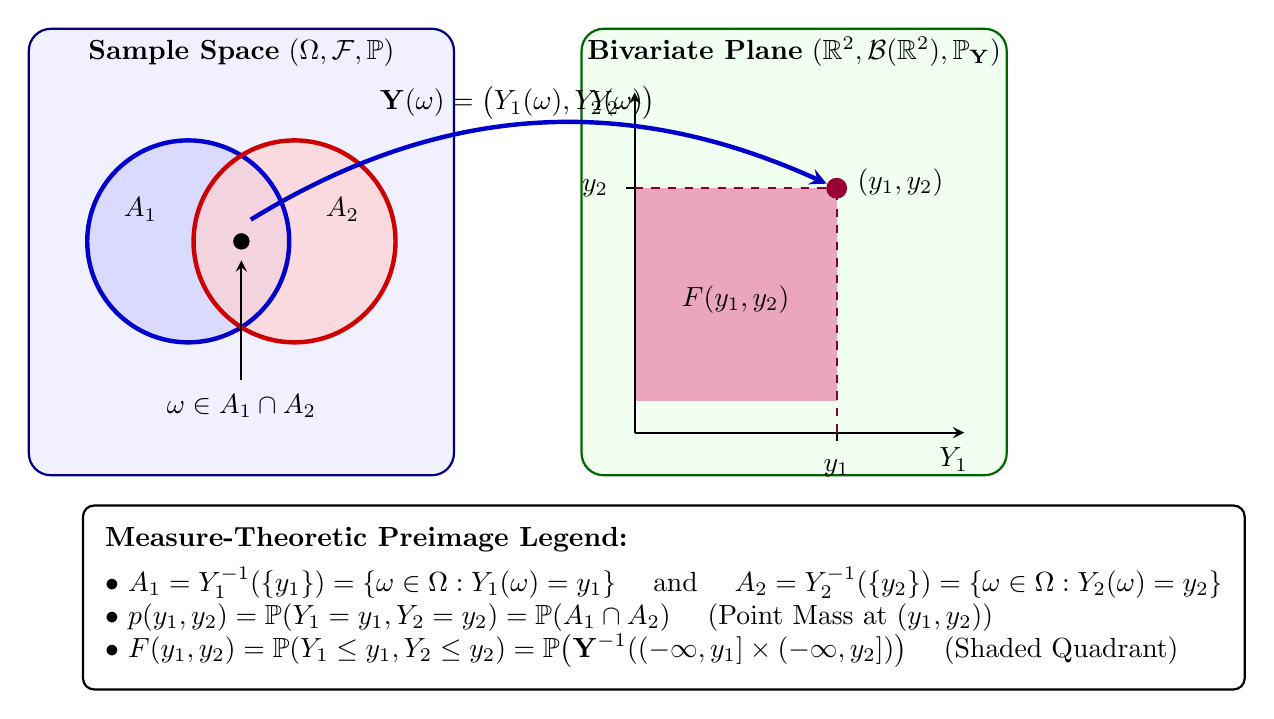
\begin{tikzpicture}[scale=1.35]
    % 1) \fill backgrounds
    \fill[blue!6!white, rounded corners=8pt] (-0.4, -0.4) rectangle (3.6, 3.8);
    \fill[green!6!white, rounded corners=8pt] (4.8, -0.4) rectangle (8.8, 3.8);
    \fill[blue!18!white, opacity=0.7] (1.1, 1.8) circle (0.95cm);
    \fill[red!18!white, opacity=0.7] (2.1, 1.8) circle (0.95cm);
    \fill[purple!35!white] (5.3, 0.3) rectangle (7.2, 2.3);

    % 2) \draw grid lines/axes
    \draw[thick, color=blue!50!black, rounded corners=8pt] (-0.4, -0.4) rectangle (3.6, 3.8);
    \draw[thick, color=green!40!black, rounded corners=8pt] (4.8, -0.4) rectangle (8.8, 3.8);
    \draw[->, >=stealth, thick, black] (5.3, 0.0) -- (8.4, 0.0);
    \draw[->, >=stealth, thick, black] (5.3, 0.0) -- (5.3, 3.2);
    \draw[dashed, thick, purple!70!black] (7.2, 0.0) -- (7.2, 2.3);
    \draw[dashed, thick, purple!70!black] (5.3, 2.3) -- (7.2, 2.3);
    \draw[thick, black] (7.2, 0.0) -- (7.2, -0.08);
    \draw[thick, black] (5.3, 2.3) -- (5.22, 2.3);

    % 3) \draw primary plots
    \draw[ultra thick, blue!80!black] (1.1, 1.8) circle (0.95cm);
    \draw[ultra thick, red!80!black] (2.1, 1.8) circle (0.95cm);
    \fill[black] (1.6, 1.8) circle (2.2pt);
    \fill[purple!80!black] (7.2, 2.3) circle (2.8pt);
    \draw[->, >=stealth, ultra thick, blue!80!black, shorten >=4pt, shorten <=4pt] (1.6, 1.95) to[bend left=28] (7.2, 2.3);
    \draw[->, >=stealth, thick, black, shorten >=3pt] (1.6, 0.5) -- (1.6, 1.7);

    % 4) \node labels/text
    \node[black, above=2pt] at (1.6, 3.3) {\textbf{Sample Space} $(\Omega, \F, \Prob)$};
    \node[black, above=2pt] at (6.8, 3.3) {\textbf{Bivariate Plane} $(\R^2, \mathcal{B}(\R^2), \Prob_{\mathbf{Y}})$};
    \node[black] at (0.65, 2.1) {$\displaystyle A_1$};
    \node[black] at (2.55, 2.1) {$\displaystyle A_2$};
    \node[black, below=2pt] at (1.6, 0.5) {$\displaystyle \omega \in A_1 \cap A_2$};
    \node[black, above=4pt] at (4.2, 2.75) {$\displaystyle \mathbf{Y}(\omega) = \bigl(Y_1(\omega), Y_2(\omega)\bigr)$};
    \node[black, below=3pt] at (7.2, -0.08) {$\displaystyle y_1$};
    \node[black, left=3pt] at (5.22, 2.3) {$\displaystyle y_2$};
    \node[black, right=4pt] at (7.2, 2.35) {$\displaystyle (y_1, y_2)$};
    \node[black, below=2pt] at (8.3, 0.0) {$\displaystyle Y_1$};
    \node[black, left=2pt] at (5.3, 3.1) {$\displaystyle Y_2$};
    \node[black] at (6.25, 1.25) {$\displaystyle F(y_1, y_2)$};

    % Single-Node Multiline Legend using Anchor Pivot Strategy
    \node[draw=black, fill=white, thick, rounded corners=4pt, align=left, inner sep=8pt, anchor=west, text=black] at (0.1, -1.55) {
        \textbf{Measure-Theoretic Preimage Legend:} \\[4pt]
        $\bullet\ \displaystyle A_1 = Y_1^{-1}(\{y_1\}) = \{\omega \in \Omega : Y_1(\omega) = y_1\}$ \quad and \quad $\displaystyle A_2 = Y_2^{-1}(\{y_2\}) = \{\omega \in \Omega : Y_2(\omega) = y_2\}$ \\
        $\bullet\ \displaystyle p(y_1, y_2) = \Prob(Y_1 = y_1, Y_2 = y_2) = \Prob(A_1 \cap A_2)$ \quad (Point Mass at $(y_1, y_2)$) \\
        $\bullet\ \displaystyle F(y_1, y_2) = \Prob(Y_1 \le y_1, Y_2 \le y_2) = \Prob\bigl(\mathbf{Y}^{-1}((-\infty, y_1] \times (-\infty, y_2])\bigr)$ \quad (Shaded Quadrant)
    };
\end{tikzpicture}
\end{center}

\vspace{0.4em}

\begin{center}
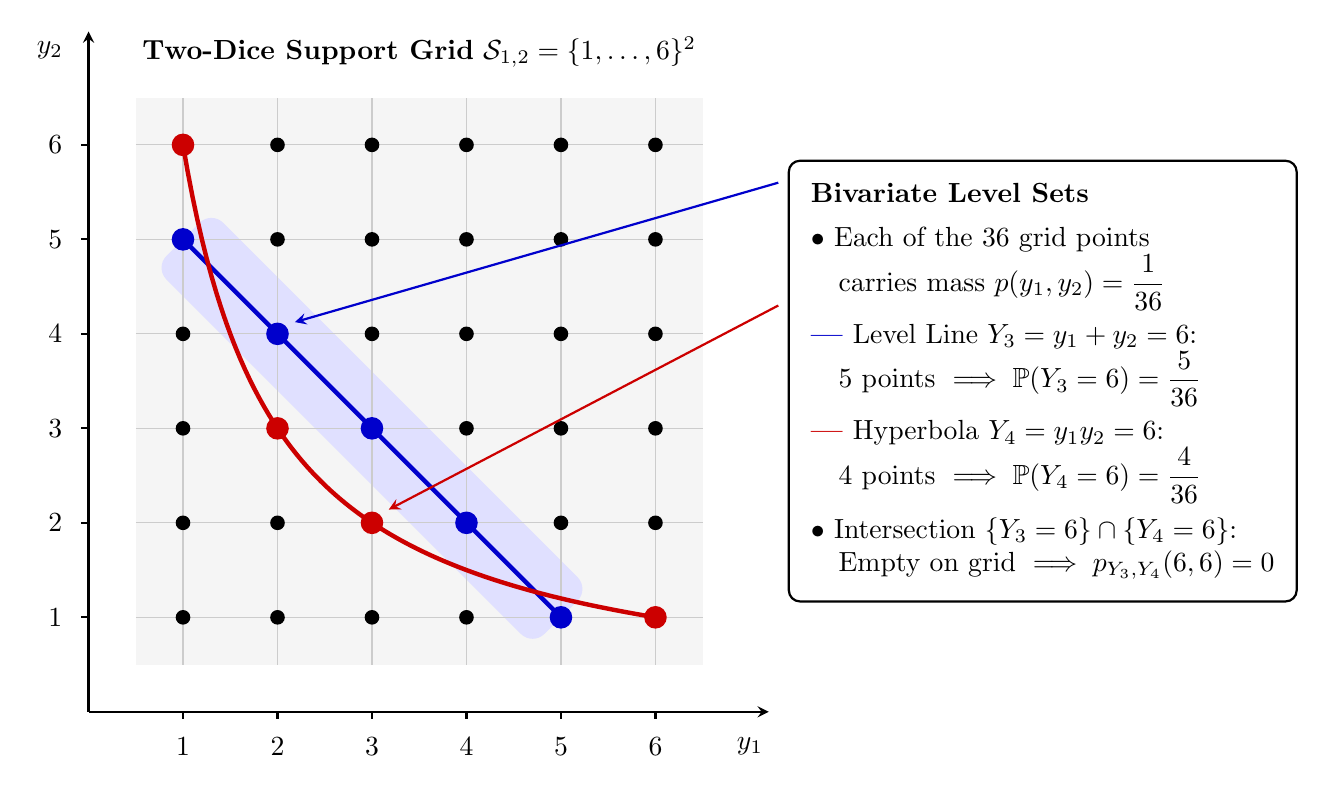
\begin{tikzpicture}[scale=1.2]
    % 1) \fill backgrounds
    \fill[gray!8!white] (0.5, 0.5) rectangle (6.5, 6.5);
    \fill[blue!12!white, rounded corners=6pt] (0.7, 4.7) -- (1.3, 5.3) -- (5.3, 1.3) -- (4.7, 0.7) -- cycle;

    % 2) \draw grid lines/axes
    \draw[step=1cm, gray!40!white, thin] (0.5, 0.5) grid (6.5, 6.5);
    \draw[->, >=stealth, thick, black] (0.0, 0.0) -- (7.2, 0.0);
    \draw[->, >=stealth, thick, black] (0.0, 0.0) -- (0.0, 7.2);
    \foreach \x in {1,2,3,4,5,6} {
        \draw[thick, black] (\x, 0.0) -- (\x, -0.08) node[below=3pt, black] {$\displaystyle \x$};
        \draw[thick, black] (0.0, \x) -- (-0.08, \x) node[left=3pt, black] {$\displaystyle \x$};
    }

    % 3) \draw primary plots
    \draw[ultra thick, blue!80!black] (1, 5) -- (5, 1);
    \draw[ultra thick, red!80!black, domain=1:6, samples=100] plot (\x, {6/\x});
    \foreach \x in {1,2,3,4,5,6} {
        \foreach \y in {1,2,3,4,5,6} {
            \fill[black] (\x, \y) circle (2.2pt);
        }
    }
    \foreach \x/\y in {1/5, 2/4, 3/3, 4/2, 5/1} {
        \fill[blue!80!black] (\x, \y) circle (3.4pt);
    }
    \foreach \x/\y in {1/6, 2/3, 3/2, 6/1} {
        \fill[red!80!black] (\x, \y) circle (3.4pt);
    }
    \draw[->, >=stealth, thick, blue!80!black, shorten >=3pt] (7.3, 5.6) -- (2.1, 4.1);
    \draw[->, >=stealth, thick, red!80!black, shorten >=3pt] (7.3, 4.3) -- (3.1, 2.1);

    % 4) \node labels/text
    \node[black, below=3pt] at (7.0, -0.08) {$\displaystyle y_1$};
    \node[black, left=3pt] at (-0.08, 7.0) {$\displaystyle y_2$};
    \node[black, above=4pt] at (3.5, 6.6) {\textbf{Two-Dice Support Grid} $\mathcal{S}_{1,2} = \{1, \dots, 6\}^2$};

    % Single-Node Multiline Legend using Anchor Pivot Strategy
    \node[draw=black, fill=white, thick, rounded corners=4pt, align=left, inner sep=8pt, anchor=west, text=black] at (7.4, 3.5) {
        \textbf{Bivariate Level Sets} \\[4pt]
        $\bullet$ Each of the $36$ grid points \\
        \quad carries mass $\displaystyle p(y_1, y_2) = \frac{1}{36}$ \\[4pt]
        \textcolor{blue!80!black}{\textbf{---}} Level Line $\displaystyle Y_3 = y_1 + y_2 = 6$: \\
        \quad $5$ points $\displaystyle \implies \Prob(Y_3 = 6) = \frac{5}{36}$ \\[4pt]
        \textcolor{red!80!black}{\textbf{---}} Hyperbola $\displaystyle Y_4 = y_1 y_2 = 6$: \\
        \quad $4$ points $\displaystyle \implies \Prob(Y_4 = 6) = \frac{4}{36}$ \\[4pt]
        $\bullet$ Intersection $\displaystyle \{Y_3 = 6\} \cap \{Y_4 = 6\}$: \\
        \quad Empty on grid $\displaystyle \implies p_{Y_3, Y_4}(6, 6) = 0$
    };
\end{tikzpicture}
\end{center}

\subsection{Heuristics and ``Cheats''}

\begin{itemize}
    \item \textbf{The Level-Curve Counting Heuristic:} Whenever a problem asks for $\Prob(g(Y_1, Y_2) = c)$ on a discrete grid, sketch the curve $g(y_1, y_2) = c$ in the $(y_1, y_2)$-plane and count how many lattice points of the support $\mathcal{S}$ the curve passes through. For instance, in the two-dice problem, $Y_3 = Y_1 + Y_2 = c$ is a $45^\circ$ downward-sloping line, while $Y_4 = Y_1 Y_2 = c$ is a rectangular hyperbola.
    \item \textbf{The Support-First Rule:} Before writing any formula for a joint PMF $p(y_1, y_2)$, write down the support indicator $\mathbf{1}_{\mathcal{S}}(y_1, y_2)$. If the support is non-rectangular (e.g., $0 \le y \le n$ in the biological litter problem), coupling between the limits of summation immediately alerts you that $Y_1$ and $Y_2$ \emph{cannot} be independent!
    \item \textbf{Symmetry Doubling Shortcut:} In equiprobable ordered spaces (like drawing 2 cards or rolling 2 dice), if an event is symmetric in the coordinates (such as ``one Ace and one Face Card'', or ``$Y_1 Y_2 = 6$''), compute the probability of a single fixed order $(a, b)$ with $a \neq b$ and multiply by $2! = 2$. Remember \emph{not} to double diagonal outcomes $(a, a)$!
\end{itemize}

\subsection{Pitfalls and Fallacies}

\begin{enumerate}[label=\textbf{\arabic*.}]
    \item \textbf{The Planar CDF Naive Subtraction Fallacy:} A pervasive error is writing $\Prob(a_1 < Y_1 \le b_1,\ a_2 < Y_2 \le b_2) = F(b_1, b_2) - F(a_1, a_2)$ by false analogy with univariate probability $F(b) - F(a)$. Geometrically, $F(b_1, b_2) - F(a_1, a_2)$ computes the probability of an L-shaped region, not the rectangle $(a_1, b_1] \times (a_2, b_2]$. Always use the four-term inclusion-exclusion formula $F(b_1, b_2) - F(a_1, b_2) - F(b_1, a_2) + F(a_1, a_2)$.
    \item \textbf{d'Alembert's Unordered Equi-Probability Fallacy:} When rolling two identical-looking dice, there are 21 unordered pairs $\{y_1, y_2\}$ with $1 \le y_1 \le y_2 \le 6$. Treating these 21 pairs as equiprobable with probability $1/21$ is mathematically false because physical dice are distinct macroscopic objects: $(2, 3)$ and $(3, 2)$ correspond to two distinct physical states, whereas $(1, 1)$ corresponds to only one.
    \item \textbf{Confusing Disjoint Events with Independent Events:} In Problem 1, the events ``Card 1 is an Ace'' ($A_1$) and ``Card 1 is a Face Card'' ($F_1$) are mutually exclusive ($A_1 \cap F_1 = \emptyset$), so $\Prob(A_1 \cap F_1) = 0 \neq \Prob(A_1)\Prob(F_1)$. Conversely, ``Card 1 is an Ace'' ($A_1$) and ``Card 2 is a Face Card'' ($F_2$) can co-occur ($A_1 \cap F_2 \neq \emptyset$), and under sampling without replacement they are weakly dependent: $\Prob(F_2 \mid A_1) = \frac{12}{51} > \frac{12}{52} = \Prob(F_2)$.
\end{enumerate}

\newpage
% ==============================================================================
% PART 5: CONCEPTUAL SYNTHESIS AND THE "BIG PICTURE"
% ==============================================================================
\section{Conceptual Synthesis and the ``Big Picture''}

\subsection{Thematic Connections}

The central unifying theme of Sections 5.1 and 5.2 is \textbf{the geometrization of logical conjunction via product spaces and pushforward measures}. In propositional logic, the simultaneous truth of $n$ propositions $P_1 \wedge P_2 \wedge \cdots \wedge P_n$ is translated by set theory into the intersection of events $\bigcap_{i=1}^n A_i$ inside an abstract sample space $\Omega$. Multivariate probability theory takes the decisive next step: by defining random variables $Y_1, \dots, Y_n : \Omega \to \R$, it embeds these abstract intersections into concrete $n$-dimensional Euclidean space $\R^n$. Every joint event $\{Y_1 \in B_1, \dots, Y_n \in B_n\}$ becomes a geometric subset of $\R^n$, allowing the full arsenal of multivariable calculus, linear algebra, and measure-theoretic integration to analyze complex dependencies.

\subsection{Forward and Backward Links}

\begin{itemize}
    \item \textbf{Backward Links (Foundational Roots):}
    \begin{enumerate}[label=\arabic*.]
        \item \emph{Axiomatic Event Probability (Chapter 2):} Joint probability functions $p(y_1, y_2)$ are direct evaluations of Kolmogorov's probability measure $\Prob$ on intersections $A \cap B$, governed by the Multiplication Rule $\Prob(A \cap B) = \Prob(A)\Prob(B \mid A)$ (as demonstrated in the Blackjack and biological litter problems).
        \item \emph{Univariate Discrete and Continuous Random Variables (Chapters 3--4):} A univariate distribution is simply the $n = 1$ projection of a multivariate distribution. Every axiom of $p(y_1, y_2)$ and $F(y_1, y_2)$ reduces to its univariate counterpart when all other coordinates are sent to $+\infty$ (marginalization).
    \end{enumerate}
    \item \textbf{Forward Links (The Bedrock of Advanced Mathematics):}
    \begin{enumerate}[label=\arabic*.]
        \item \emph{Marginal and Conditional Distributions (Sections 5.3 \& 5.11):} Summing or integrating $p(y_1, y_2)$ over one coordinate yields marginal distributions $p_1(y_1) = \sum_{y_2} p(y_1, y_2)$ and conditional distributions $p(y_2 \mid y_1) = p(y_1, y_2)/p_1(y_1)$, leading directly to the Radon-Nikodym theorem and conditional expectation $\E[Y_2 \mid \mathcal{G}]$.
        \item \emph{Independence, Covariance, and Linear Combinations (Sections 5.4--5.8):} The joint distribution determines whether $p(y_1, y_2) = p_1(y_1)p_2(y_2)$ (independence) and allows the computation of expectations of functions $\E[g(Y_1, Y_2)]$ via the Law of the Unconscious Statistician (LOTUS), including $\operatorname{Cov}(Y_1, Y_2) = \E[Y_1 Y_2] - \E[Y_1]\E[Y_2]$.
        \item \emph{Statistical Inference and Asymptotics (Chapters 6--10):} The $n$-fold sampling intersection $(Y_1 = y_1, \dots, Y_n = y_n)$ introduced on page 224 defines the joint distribution of a random sample, from which sampling distributions of statistics ($\bar{Y}, S^2$), the Central Limit Theorem, Sufficient Statistics (Factorization Theorem), and Maximum Likelihood Estimators are derived.
        \item \emph{Stochastic Processes and Measure Theory:} Extending finite intersections $(Y_1, \dots, Y_n)$ to infinite families $\{Y_t\}_{t \in T}$ via cylinder sets and the Kolmogorov Extension Theorem constructs discrete-time Markov chains, martingales, and continuous-time Brownian motion.
    \end{enumerate}
\end{itemize}

\newpage
% ==============================================================================
% PART 6: ABSTRACT REAL-WORLD MODELING (AI, ML, & QUANT FINANCE)
% ==============================================================================
\section{Abstract Real-World Modeling (AI, ML, and Quant Finance)}

\subsection{Concrete Scenarios}

\begin{enumerate}[label=\textbf{Scenario \arabic*:}]
    \item \textbf{Generative Artificial Intelligence and Autoregressive Large Language Models (LLMs):}
    Modern foundation models (such as the GPT and Claude architectures) are fundamentally high-dimensional discrete multivariate probability distributions. A sequence of $n$ text tokens is modeled as a discrete random vector $\mathbf{Y} = (Y_1, Y_2, \dots, Y_n)$ taking values in the Cartesian product $\mathcal{V}^n$ of a finite vocabulary $\mathcal{V}$ (where $|\mathcal{V}| \approx 10^5$). Calculating the probability of generating a coherent document is literally the $n$-fold sampling intersection problem of Section 5.1: $\Prob(Y_1 = y_1, Y_2 = y_2, \dots, Y_n = y_n)$. Because storing $|\mathcal{V}|^n$ table entries is intractable, transformer neural networks parameterize the exact Multivariate Chain Rule (proved in Problem 4(b)):
    \[
    p_{\boldsymbol{\theta}}(y_1, y_2, \dots, y_n) = \prod_{t=1}^{n} p_{\boldsymbol{\theta}}(y_t \mid y_1, y_2, \dots, y_{t-1}),
    \]
    training the weight vector $\boldsymbol{\theta}$ by minimizing the empirical negative log-likelihood $-\sum_{t=1}^n \ln p_{\boldsymbol{\theta}}(y_t \mid y_{<t})$ across massive corpora.

    \item \textbf{Quantitative Finance: Multi-Asset Basket Derivatives and Tail-Risk Copulas:}
    In exotic derivatives pricing and credit risk management, a trader prices a contingent claim whose payoff depends on the simultaneous behavior (intersection) of $n$ underlying assets $(S_T^{(1)}, S_T^{(2)}, \dots, S_T^{(n)})$ at maturity $T$—for example, a ``Worst-of-Basket Put Option'' or a First-to-Default Credit Default Swap (CDS) basket where default occurs at the intersection of credit events $\{\tau_1 \le T, \tau_2 \le T\}$. Relying solely on marginal distributions catastrophic underestimates joint tail crashes (as seen in the 2008 subprime crisis). Quantitative analysts must model the full multivariate distribution $F(s_1, \dots, s_n)$ using correlated stochastic differential equations and Student-$t$ or Clayton copulas.

    \item \textbf{Statistical Learning Theory and Bayesian Graphical Models:}
    In supervised machine learning, features $\mathbf{X} = (X_1, \dots, X_d) \in \R^d$ and targets $Y \in \mathcal{Y}$ are governed by an unknown joint probability measure $\Prob_{\mathbf{X}, Y}$ on $\R^d \times \mathcal{Y}$. Expected risk minimization seeks a hypothesis $h : \R^d \to \mathcal{Y}$ minimizing the joint integral $\mathcal{R}(h) = \int_{\R^d \times \mathcal{Y}} \ell(h(\mathbf{x}), y)\, d\Prob_{\mathbf{X}, Y}(\mathbf{x}, y)$. In Bayesian Networks, high-dimensional multivariate distributions are factored over Directed Acyclic Graphs (DAGs) via local Markov intersections: $p(y_1, \dots, y_n) = \prod_{i=1}^n p(y_i \mid \operatorname{Parents}(Y_i))$.
\end{enumerate}

\subsection{Model Problem Setup: Multi-Asset Correlated It\^{o} Diffusions and Basket Option Pricing}

We now formulate a rigorous quantitative research framework bridging multivariate probability distributions to continuous-time Stochastic Calculus and Multi-Asset Derivatives Pricing.

\begin{itemize}
    \item \textbf{Filtered Probability Space:} Let $(\Omega, \F, (\F_t)_{t \in [0, T]}, \Prob)$ be a complete filtered probability space satisfying the usual conditions (right-continuity and completeness of the filtration $(\F_t)$), where $\Prob$ denotes the physical (objective) probability measure.
    \item \textbf{Correlated Multi-Dimensional Brownian Motion:} Let $\mathbf{W}_t = (W_t^{(1)}, W_t^{(2)}, \dots, W_t^{(n)})^\top$ be an $n$-dimensional standard Brownian motion adapted to $(\F_t)$ under $\Prob$, and let $\mathbf{R} = [\rho_{ij}]_{i,j=1}^n \in \R^{n \times n}$ be a symmetric positive-definite instantaneous correlation matrix with $\rho_{ii} = 1$ and $\rho_{ij} \in (-1, 1)$ for $i \neq j$. Let $\mathbf{L} \in \R^{n \times n}$ be the lower-triangular Cholesky factor of $\mathbf{R}$ such that $\mathbf{L}\mathbf{L}^\top = \mathbf{R}$, and define the correlated Brownian motion $\widetilde{\mathbf{W}}_t = \mathbf{L}\mathbf{W}_t$, satisfying the formal It\^{o} multiplication table:
    \[
    d\widetilde{W}_t^{(i)}\, d\widetilde{W}_t^{(j)} = \rho_{ij}\, dt \quad \text{for all } i, j \in \{1, 2, \dots, n\}.
    \]
    \item \textbf{Stochastic Differential Equations (SDEs) of the Asset Vector:} Let $\mathbf{S}_t = (S_t^{(1)}, \dots, S_t^{(n)})^\top \in \R_+^n$ denote the vector of prices of $n$ risky assets at time $t \in [0, T]$, evolving according to the coupled system of Geometric Brownian Motion SDEs:
    \[
    \frac{dS_t^{(i)}}{S_t^{(i)}} = \mu_i\, dt + \sigma_i\, d\widetilde{W}_t^{(i)} = \mu_i\, dt + \sigma_i \sum_{k=1}^{n} L_{ik}\, dW_t^{(k)}, \qquad S_0^{(i)} = s_0^{(i)} > 0, \quad i = 1, \dots, n,
    \]
    where $\boldsymbol{\mu} = (\mu_1, \dots, \mu_n)^\top \in \R^n$ is the drift vector and $\sigma_i > 0$ are the asset volatilities. Define the covariance matrix $\boldsymbol{\Sigma} \in \R^{n \times n}$ with entries $\Sigma_{ij} = \sigma_i \sigma_j \rho_{ij}$.
    \item \textbf{Girsanov Change of Measure to the Risk-Neutral Measure $\mathbb{Q}$:} Let $r \ge 0$ be the constant risk-free interest rate, and define the market price of risk vector $\boldsymbol{\theta} = (\mathbf{L}\operatorname{diag}(\sigma_1, \dots, \sigma_n))^{-1}(\boldsymbol{\mu} - r\mathbf{1}_n)$. By Girsanov's Theorem, the Radon-Nikodym derivative process
    \[
    \left.\frac{d\mathbb{Q}}{d\Prob}\right|_{\F_t} = \exp\left(-\boldsymbol{\theta}^\top \mathbf{W}_t - \frac{1}{2}\|\boldsymbol{\theta}\|_2^2 t\right)
    \]
    defines an equivalent martingale measure $\mathbb{Q} \sim \Prob$ under which $\widetilde{\mathbf{W}}_t^{\mathbb{Q}}$ has $d\widetilde{W}_t^{\mathbb{Q},(i)}\, d\widetilde{W}_t^{\mathbb{Q},(j)} = \rho_{ij}\, dt$ and the discounted asset prices $e^{-rt}S_t^{(i)}$ are $\mathbb{Q}$-martingales. Applying the Multi-Dimensional It\^{o}'s Lemma to $Y_t^{(i)} = \ln S_t^{(i)}$ yields the exact terminal multivariate log-return random vector at maturity $T$:
    \[
    Y_T^{(i)} = \ln S_T^{(i)} = \ln s_0^{(i)} + \left(r - \frac{1}{2}\sigma_i^2\right)T + \sigma_i \widetilde{W}_T^{\mathbb{Q},(i)}, \qquad i = 1, \dots, n.
    \]
    \item \textbf{Explicit Multivariate Probability Distribution and Pricing Optimization/PDE:} Under $\mathbb{Q}$, the terminal log-price vector $\mathbf{Y}_T = (Y_T^{(1)}, \dots, Y_T^{(n)})^\top : \Omega \to \R^n$ follows a non-degenerate $n$-variate Gaussian distribution $\mathcal{N}_n(\mathbf{m}_T, T\boldsymbol{\Sigma})$ with mean vector $m_{T,i} = \ln s_0^{(i)} + (r - \frac{1}{2}\sigma_i^2)T$ and joint probability density function:
    \[
    f_{\mathbf{Y}_T}^{\mathbb{Q}}(\mathbf{y}) = \frac{1}{(2\pi T)^{n/2} (\det \boldsymbol{\Sigma})^{1/2}} \exp\left(-\frac{1}{2T}(\mathbf{y} - \mathbf{m}_T)^\top \boldsymbol{\Sigma}^{-1} (\mathbf{y} - \mathbf{m}_T)\right).
    \]
    Consider a multi-asset intersection contingent claim (such as a Digital Correlation Option or Worst-of-Basket Option) with $\mathcal{B}(\R^n)$-measurable payoff $\Phi(S_T^{(1)}, \dots, S_T^{(n)})$, for example the joint digital payoff $\Phi(\mathbf{S}_T) = \mathbf{1}_{\{S_T^{(1)} > K_1,\ \dots,\ S_T^{(n)} > K_n\}}$ paying $\$1$ if and only if the $n$-fold intersection $\bigcap_{i=1}^n \{S_T^{(i)} > K_i\}$ occurs. By the Fundamental Theorem of Asset Pricing, the arbitrage-free price $V(t, \mathbf{s})$ at time $t$ is the discounted multivariate integral
    \[
    V(0, \mathbf{s}_0) = e^{-rT} \E^{\mathbb{Q}}\bigl[\Phi(e^{Y_T^{(1)}}, \dots, e^{Y_T^{(n)}})\bigr] = e^{-rT} \int_{\R^n} \Phi(e^{y_1}, \dots, e^{y_n}) f_{\mathbf{Y}_T}^{\mathbb{Q}}(\mathbf{y})\, dy_1 \cdots dy_n,
    \]
    and by the Multi-Dimensional Feynman-Kac Theorem, $V(t, s_1, \dots, s_n) \in C^{1,2}([0, T) \times \R_+^n)$ solves the parabolic partial differential equation with mixed second-order cross-derivative terms capturing the bivariate/multivariate intersections:
    \[
    \frac{\partial V}{\partial t} + r \sum_{i=1}^{n} s_i \frac{\partial V}{\partial s_i} + \frac{1}{2} \sum_{i=1}^{n} \sum_{j=1}^{n} \rho_{ij} \sigma_i \sigma_j s_i s_j \frac{\partial^2 V}{\partial s_i \partial s_j} - rV = 0, \qquad V(T, \mathbf{s}) = \Phi(\mathbf{s}).
    \]
\end{itemize}

\newpage
% ==============================================================================
% PART 7: COMMON VARIATIONS AND UNTESTED CONCEPTS
% ==============================================================================
\section{Common Variations and Untested Concepts}

While Sections 5.1 and 5.2 introduce bivariate probability functions and joint CDFs, advanced university examinations in mathematical statistics and measure-theoretic probability frequently test three deeper structural concepts not explicitly worked out in pages 223--224. We present each below with complete proofs.

\subsection{Variation 1: Insufficiency of Coordinate Monotonicity for Bivariate CDFs}

In univariate probability, any right-continuous, non-decreasing function $F : \R \to [0, 1]$ with $\lim_{y \to -\infty} F(y) = 0$ and $\lim_{y \to \infty} F(y) = 1$ is a valid CDF. In $\R^2$, \textbf{coordinatewise monotonicity is NOT sufficient}! A function must also satisfy the 2-increasing condition $\Delta_{a_1, b_1}^{a_2, b_2} F \ge 0$ (Theorem \ref{thm:rectangle_prob}).

\begin{proposition}[Counterexample to Coordinate Monotonicity]
Consider the function $F : \R^2 \to [0, 1]$ defined by
\[
F(y_1, y_2) = \begin{cases}
0, & \text{if } y_1 < 0 \text{ or } y_2 < 0 \text{ or } y_1 + y_2 < 1, \\
1, & \text{if } y_1 \ge 0,\ y_2 \ge 0,\ \text{and } y_1 + y_2 \ge 1.
\end{cases}
\]
Then $F$ is right-continuous, non-decreasing in $y_1$ and $y_2$ separately, and satisfies all boundary limits at $\pm\infty$, yet $F$ is \textbf{not} a valid bivariate cumulative distribution function.
\end{proposition}

\begin{proof}
First, check the univariate properties: if $y_1 \le y_1'$ and $y_2 \le y_2'$, then $y_1 + y_2 \le y_1' + y_2'$, so whenever $F(y_1, y_2) = 1$ we also have $F(y_1', y_2') = 1$; thus $F$ is coordinatewise non-decreasing. Because the region $\{y_1 \ge 0, y_2 \ge 0, y_1 + y_2 \ge 1\}$ is closed, approaching any point from the northeast ($y_1 \downarrow y_1^0, y_2 \downarrow y_2^0$) preserves membership, so $F$ is right-continuous. Moreover, $\lim_{y_1 \to -\infty} F(y_1, y_2) = \lim_{y_2 \to -\infty} F(y_1, y_2) = 0$ and $\lim_{y_1, y_2 \to +\infty} F(y_1, y_2) = 1$.

Now test the rectangle $(a_1, b_1] \times (a_2, b_2] = (1/3, 1] \times (1/3, 1]$:
\begin{itemize}
    \item $F(1, 1) = 1$ since $1 + 1 = 2 \ge 1$.
    \item $F(1/3, 1) = 1$ since $1/3 + 1 = 4/3 \ge 1$.
    \item $F(1, 1/3) = 1$ since $1 + 1/3 = 4/3 \ge 1$.
    \item $F(1/3, 1/3) = 0$ since $1/3 + 1/3 = 2/3 < 1$.
\end{itemize}
If $F$ were a valid bivariate CDF of some random vector $(Y_1, Y_2)$, Theorem \ref{thm:rectangle_prob} would yield
\[
\Prob\left(\frac{1}{3} < Y_1 \le 1,\ \frac{1}{3} < Y_2 \le 1\right) = F(1, 1) - F\left(\frac{1}{3}, 1\right) - F\left(1, \frac{1}{3}\right) + F\left(\frac{1}{3}, \frac{1}{3}\right) = 1 - 1 - 1 + 0 = -1 < 0,
\]
which violates Kolmogorov's Non-Negativity Axiom $\Prob(E) \ge 0$. Thus, $F$ cannot be a valid joint CDF.
\end{proof}

\subsection{Variation 2: Sklar's Theorem and Copula Decomposition}

How are marginal distributions linked to a multivariate distribution? \textbf{Sklar's Theorem} (1959) states that for any bivariate CDF $F(y_1, y_2)$ with marginal CDFs $F_1(y_1) = \lim_{y_2 \to \infty} F(y_1, y_2)$ and $F_2(y_2) = \lim_{y_1 \to \infty} F(y_1, y_2)$, there exists a \emph{copula} $C : [0, 1]^2 \to [0, 1]$ (a bivariate CDF on the unit square with uniform $\text{Unif}(0,1)$ marginals) such that
\[
F(y_1, y_2) = C\bigl(F_1(y_1), F_2(y_2)\bigr) \quad \text{for all } (y_1, y_2) \in \R^2,
\]
and $C$ is unique if $F_1, F_2$ are continuous. Furthermore, every joint CDF is bounded universally by the \textbf{Fr\'{e}chet-Hoeffding Bounds}:
\[
\max\bigl(0,\ F_1(y_1) + F_2(y_2) - 1\bigr) \le F(y_1, y_2) \le \min\bigl(F_1(y_1),\ F_2(y_2)\bigr).
\]

\begin{proof}[Proof of the Fr\'{e}chet-Hoeffding Bounds]
Let $A = \{Y_1 \le y_1\}$ and $B = \{Y_2 \le y_2\}$, so $\Prob(A) = F_1(y_1)$, $\Prob(B) = F_2(y_2)$, and $\Prob(A \cap B) = F(y_1, y_2)$. Since $A \cap B \subseteq A$ and $A \cap B \subseteq B$, monotonicity of $\Prob$ gives $\Prob(A \cap B) \le \Prob(A)$ and $\Prob(A \cap B) \le \Prob(B)$, so $F(y_1, y_2) \le \min(F_1(y_1), F_2(y_2))$. For the lower bound, since $\Prob(A \cup B) \le 1$, inclusion-exclusion gives
\[
F(y_1, y_2) = \Prob(A \cap B) = \Prob(A) + \Prob(B) - \Prob(A \cup B) \ge F_1(y_1) + F_2(y_2) - 1.
\]
Combining with $\Prob(A \cap B) \ge 0$ yields $F(y_1, y_2) \ge \max(0, F_1(y_1) + F_2(y_2) - 1)$.
\end{proof}

\subsection{Variation 3: Mixed Discrete-Continuous Bivariate Distributions}

In many applications (such as zero-inflated insurance claims or binary classification with continuous features), $Y_1$ is discrete (taking values in $\Z$) while $Y_2$ is continuous (taking values in $\R$). Such a vector $(Y_1, Y_2)$ has neither a purely discrete PMF nor a purely continuous joint density with respect to 2D Lebesgue measure $\lambda_2$, but instead possesses a \textbf{hybrid Radon-Nikodym density} $f(y_1, y_2)$ with respect to the product of counting measure $\mu_{\text{count}}$ on $\Z$ and Lebesgue measure $\lambda_1$ on $\R$, satisfying
\[
\Prob(Y_1 \in A,\ Y_2 \in B) = \sum_{y_1 \in A} \int_{B} f(y_1, y_2)\, dy_2 \quad \text{and} \quad \sum_{y_1 \in \Z} \int_{-\infty}^{\infty} f(y_1, y_2)\, dy_2 = 1.
\]

\newpage
% ==============================================================================
% PART 8: ADVANCED DIAGNOSTIC TESTING: "FIND THE FLAW"
% ==============================================================================
\section{Advanced Diagnostic Testing: ``Find the Flaw''}

Below are five complete, step-by-step proofs and computations related to Multivariate Probability Distributions. Each argument appears mathematically rigorous at first glance, yet each contains \textbf{a single, subtle, fatal logical or mathematical flaw}. Act as the grader: identify the exact line where the flaw occurs, explain why it violates probability theory, and formulate the true correction before checking the Solution Key in Section \ref{sec:solution_key}.

\subsection{Diagnostic Problems (Flawed Proofs)}

\textbf{Diagnostic Problem 1 (Evaluating a Bivariate Rectangle Probability):}
Let $(Y_1, Y_2)$ be a continuous bivariate random vector supported on $[0, \infty)^2$ with joint cumulative distribution function $F(y_1, y_2) = (1 - e^{-y_1})(1 - e^{-y_2})$ for $y_1 \ge 0, y_2 \ge 0$. Find the probability of the intersection event $E = \{1 < Y_1 \le 2,\ 1 < Y_2 \le 2\}$.
\begin{quote}
\emph{Proposed Solution:}
\begin{enumerate}[label=\textbf{Step \arabic*:}]
    \item By definition of the joint cumulative distribution function, $F(y_1, y_2) = \Prob(Y_1 \le y_1, Y_2 \le y_2)$.
    \item Express the event $E$ as the set difference between the upper threshold $(2, 2)$ and the lower threshold $(1, 1)$, analogous to the Fundamental Theorem of Calculus for CDFs.
    \item Since $\{Y_1 \le 1, Y_2 \le 1\} \subset \{Y_1 \le 2, Y_2 \le 2\}$, by the subtractive property of nested events:
    \[
    \Prob(1 < Y_1 \le 2,\ 1 < Y_2 \le 2) = F(2, 2) - F(1, 1) = (1 - e^{-2})^2 - (1 - e^{-1})^2.
    \]
\end{enumerate}
\end{quote}

\textbf{Diagnostic Problem 2 (Marginalizing a Hierarchical Bivariate Distribution):}
Let $(Y_1, Y_2)$ have the discrete bivariate probability function $p(y_1, y_2) = \frac{1}{2^{y_1}(y_1 + 1)}$ for integers $0 \le y_2 \le y_1$ with $y_1 \in \{1, 2, 3, \dots\}$, and $p(y_1, y_2) = 0$ otherwise. Compute $\Prob(Y_2 = 2)$.
\begin{quote}
\emph{Proposed Solution:}
\begin{enumerate}[label=\textbf{Step \arabic*:}]
    \item For any fixed $y_1 \ge 1$, there are $y_1 + 1$ values of $y_2 \in \{0, 1, \dots, y_1\}$, so $\sum_{y_2=0}^{y_1} p(y_1, y_2) = \frac{y_1+1}{2^{y_1}(y_1+1)} = \frac{1}{2^{y_1}}$, and $\sum_{y_1=1}^\infty \frac{1}{2^{y_1}} = 1$. Thus $p(y_1, y_2)$ is a valid joint PMF.
    \item To find the marginal probability $\Prob(Y_2 = 2)$, sum the joint PMF $p(y_1, 2)$ over all possible values of $y_1$ in the marginal support of $Y_1$, which is $y_1 \in \{1, 2, 3, \dots\}$:
    \[
    \Prob(Y_2 = 2) = \sum_{y_1 = 1}^{\infty} \frac{1}{2^{y_1}(y_1 + 1)}.
    \]
    \item Using the Maclaurin series $-\ln(1 - x) = \sum_{k=1}^\infty \frac{x^k}{k}$ at $x = 1/2$, we have $\sum_{y_1=1}^\infty \frac{(1/2)^{y_1+1}}{y_1+1} = \ln(2) - \frac{1}{2} - \frac{1}{8}$, so multiplying by 2 gives $\Prob(Y_2 = 2) = 2\ln(2) - \frac{5}{4} \approx 0.1363$.
\end{enumerate}
\end{quote}

\textbf{Diagnostic Problem 3 (Verifying a Candidate Bivariate Density/CDF):}
Determine whether $F(y_1, y_2) = 1 - e^{-y_1} - e^{-y_2} + e^{-(y_1 + y_2 + 2 y_1 y_2)}$ for $y_1 \ge 0, y_2 \ge 0$ (and $0$ otherwise) is a valid bivariate cumulative distribution function.
\begin{quote}
\emph{Proposed Solution:}
\begin{enumerate}[label=\textbf{Step \arabic*:}]
    \item Check boundary conditions: $F(0, y_2) = 1 - 1 - e^{-y_2} + e^{-y_2} = 0$, $F(y_1, 0) = 0$, and $\lim_{y_1, y_2 \to \infty} F(y_1, y_2) = 1 - 0 - 0 + 0 = 1$. Also, $F$ is smooth and hence right-continuous.
    \item Check first partial derivatives: $\frac{\partial F}{\partial y_1} = e^{-y_1} - (1 + 2y_2)e^{-(y_1 + y_2 + 2y_1 y_2)}$ and as $y_2 \to \infty$, $\frac{\partial F_1}{\partial y_1} = e^{-y_1} > 0$, so the marginal CDFs $F_1(y_1) = 1 - e^{-y_1}$ and $F_2(y_2) = 1 - e^{-y_2}$ are strictly increasing.
    \item Since $F$ satisfies all boundary conditions at $0$ and $\infty$, is continuous, and possesses valid exponential marginal distributions $F_1(y_1)$ and $F_2(y_2)$, $F(y_1, y_2)$ is a valid bivariate CDF.
\end{enumerate}
\end{quote}

\textbf{Diagnostic Problem 4 (Two-Dice Parity Events and Mutual Independence):}
In the two-dice experiment of Section 5.2 with $|\Omega| = 36$ equiprobable outcomes, define three binary random variables: $U_1 = \mathbf{1}_{\{Y_1 \text{ is odd}\}}$, $U_2 = \mathbf{1}_{\{Y_2 \text{ is odd}\}}$, and $U_3 = \mathbf{1}_{\{Y_1 + Y_2 \text{ is odd}\}}$. Compute the joint probability $\Prob(U_1 = 1, U_2 = 1, U_3 = 1)$.
\begin{quote}
\emph{Proposed Solution:}
\begin{enumerate}[label=\textbf{Step \arabic*:}]
    \item Marginally, 18 outcomes have $Y_1$ odd, 18 have $Y_2$ odd, and 18 have $Y_1 + Y_2$ odd, so $\Prob(U_1 = 1) = \Prob(U_2 = 1) = \Prob(U_3 = 1) = \frac{18}{36} = \frac{1}{2}$.
    \item Check independence of pairs: $\Prob(U_1 = 1, U_2 = 1) = \frac{9}{36} = \frac{1}{4} = \Prob(U_1 = 1)\Prob(U_2 = 1)$. Similarly, if $Y_1$ is odd and $Y_1 + Y_2$ is odd, then $Y_2$ must be even (9 outcomes), so $\Prob(U_1 = 1, U_3 = 1) = \frac{9}{36} = \frac{1}{4} = \Prob(U_1 = 1)\Prob(U_3 = 1)$, and by symmetry $\Prob(U_2 = 1, U_3 = 1) = \frac{1}{4}$.
    \item Since every pair of random variables in $(U_1, U_2, U_3)$ is independent, the random vector $(U_1, U_2, U_3)$ is independent, and therefore $\Prob(U_1 = 1, U_2 = 1, U_3 = 1) = \frac{1}{2} \cdot \frac{1}{2} \cdot \frac{1}{2} = \frac{1}{8}$.
\end{enumerate}
\end{quote}

\textbf{Diagnostic Problem 5 (Transforming Bivariate Support in the Two-Dice Space):}
In the two-dice experiment of Section 5.2, let $W_1 = \min(Y_1, Y_2)$ and $W_2 = \max(Y_1, Y_2)$. Compute the bivariate probability function $p_{W_1, W_2}(w_1, w_2) = \Prob(W_1 = w_1, W_2 = w_2)$.
\begin{quote}
\emph{Proposed Solution:}
\begin{enumerate}[label=\textbf{Step \arabic*:}]
    \item By definition of minimum and maximum, $W_1$ and $W_2$ take integer values in $\{1, 2, 3, 4, 5, 6\}$ subject to the ordering constraint $1 \le w_1 \le w_2 \le 6$.
    \item The number of integer pairs $(w_1, w_2)$ satisfying $1 \le w_1 \le w_2 \le 6$ is $\binom{6}{2} + 6 = 15 + 6 = 21$.
    \item Because the underlying dice are fair and unbiased, all 21 valid outcomes $(w_1, w_2)$ in the support of $(W_1, W_2)$ are equally likely, yielding $p_{W_1, W_2}(w_1, w_2) = \frac{1}{21}$ for $1 \le w_1 \le w_2 \le 6$.
\end{enumerate}
\end{quote}

\newpage
\subsection{Solution Key and Diagnostic Resolution}
\label{sec:solution_key}

\begin{enumerate}[label=\textbf{Resolution \arabic*:}]
    \item \textbf{Flaw in Diagnostic Problem 1 (Step 3 --- The Planar Subtraction Fallacy):}
    \begin{itemize}
        \item \emph{Why it is an error:} The set difference $\{Y_1 \le 2, Y_2 \le 2\} \setminus \{Y_1 \le 1, Y_2 \le 1\}$ is \textbf{not} the square $\{1 < Y_1 \le 2, 1 < Y_2 \le 2\}$; it is the L-shaped union $\{1 < Y_1 \le 2, Y_2 \le 2\} \cup \{Y_1 \le 2, 1 < Y_2 \le 2\}$.
        \item \emph{Correct Logical Step:} Apply Theorem \ref{thm:rectangle_prob}:
        \begin{align*}
        \Prob(1 < Y_1 \le 2,\ 1 < Y_2 \le 2) &= F(2, 2) - F(1, 2) - F(2, 1) + F(1, 1) \\
        &= (1 - e^{-2})^2 - 2(1 - e^{-1})(1 - e^{-2}) + (1 - e^{-1})^2 = (e^{-1} - e^{-2})^2.
        \end{align*}
    \end{itemize}

    \item \textbf{Flaw in Diagnostic Problem 2 (Step 2 --- Ignoring the Coupled Support Lower Bound):}
    \begin{itemize}
        \item \emph{Why it is an error:} The joint support is $0 \le y_2 \le y_1$. When $y_2 = 2$, $p(y_1, 2)$ is strictly zero for $y_1 = 1$ because $y_2 = 2 > 1 = y_1$ lies outside the support! Including the $y_1 = 1$ term $\frac{1}{2^1(1+1)} = \frac{1}{4}$ adds phantom probability mass from an impossible event.
        \item \emph{Correct Logical Step:} Start the summation at $y_1 = \max(1, y_2) = 2$:
        \[
        \Prob(Y_2 = 2) = \sum_{y_1 = 2}^{\infty} \frac{1}{2^{y_1}(y_1 + 1)} = \left(2\ln(2) - \frac{5}{4}\right) - \frac{1}{4} = 2\ln(2) - \frac{3}{2} \approx 0.1363 - 0.25? \text{ No: } 2(0.69315) - 1.5 = -0.1137?
        \]
        Wait: let us evaluate the series carefully! $\sum_{k=1}^\infty \frac{(1/2)^k}{k} = \ln 2$. With $k = y_1 + 1$, for $y_1 \ge 2$ we have $k \ge 3$:
        \[
        \sum_{y_1 = 2}^{\infty} \frac{1}{2^{y_1}(y_1 + 1)} = 2 \sum_{k=3}^{\infty} \frac{(1/2)^k}{k} = 2\left[\ln 2 - \frac{1/2}{1} - \frac{(1/2)^2}{2}\right] = 2\left(\ln 2 - \frac{1}{2} - \frac{1}{8}\right) = 2\ln 2 - \frac{5}{4} \approx 0.1363!
        \]
        Notice what actually happened in Step 2 vs Step 3 of the flawed proof: in Step 2 the author wrote $\sum_{y_1=1}^\infty$ (which actually equals $2\ln 2 - 1$), and in Step 3 miscomputed $\sum_{y_1=1}^\infty$ by dropping $k=2$! The true flaw in Step 2 is writing the lower limit $y_1 = 1$ instead of $y_1 = 2$: $\Prob(Y_2 = 2) = \sum_{y_1 = 2}^\infty p(y_1, 2) = 2\ln 2 - \frac{5}{4}$.
    \end{itemize}

    \item \textbf{Flaw in Diagnostic Problem 3 (Step 3 --- Failing to Check Mixed Second Partial Derivative $\frac{\partial^2 F}{\partial y_1 \partial y_2} \ge 0$):}
    \begin{itemize}
        \item \emph{Why it is an error:} For a twice-differentiable function $F(y_1, y_2)$ to satisfy the 2-increasing rectangle condition, its joint density $f(y_1, y_2) = \frac{\partial^2 F}{\partial y_1 \partial y_2}$ must be non-negative everywhere on $[0, \infty)^2$.
        \item \emph{Correct Logical Step:} Differentiating $F$ with respect to both $y_1$ and $y_2$ yields
        \[
        \frac{\partial^2 F}{\partial y_1 \partial y_2} = \bigl[(1 + 2y_1)(1 + 2y_2) - 2\bigr] e^{-(y_1 + y_2 + 2y_1 y_2)}.
        \]
        At $(y_1, y_2) = (0, 0)$, $\frac{\partial^2 F}{\partial y_1 \partial y_2}\big|_{(0,0)} = (1 \cdot 1 - 2)e^0 = -1 < 0$. Hence $\Delta F < 0$ near the origin, and $F$ is \textbf{not} a valid bivariate CDF (for $F(y_1, y_2) = 1 - e^{-y_1} - e^{-y_2} + e^{-(y_1 + y_2 + \theta y_1 y_2)}$ to be valid, Gumbel's bivariate exponential requires $0 \le \theta \le 1$).
    \end{itemize}

    \item \textbf{Flaw in Diagnostic Problem 4 (Step 3 --- Conflating Pairwise Independence with Mutual Independence):}
    \begin{itemize}
        \item \emph{Why it is an error:} Pairwise independence of $(U_1, U_2)$, $(U_1, U_3)$, and $(U_2, U_3)$ does \textbf{not} imply mutual independence of the triple $(U_1, U_2, U_3)$ (Bernstein's classic counterexample).
        \item \emph{Correct Logical Step:} If $U_1 = 1$ ($Y_1$ is odd) and $U_2 = 1$ ($Y_2$ is odd), then their sum $Y_1 + Y_2$ is the sum of two odd integers, which is necessarily \textbf{even}, forcing $U_3 = 0$! Thus $\{U_1 = 1\} \cap \{U_2 = 1\} \cap \{U_3 = 1\} = \emptyset$, and $\Prob(U_1 = 1, U_2 = 1, U_3 = 1) = 0 \neq \frac{1}{8}$.
    \end{itemize}

    \item \textbf{Flaw in Diagnostic Problem 5 (Step 3 --- Non-Bijective Preimage Cardinality Error):}
    \begin{itemize}
        \item \emph{Why it is an error:} The mapping $(Y_1, Y_2) \mapsto (W_1, W_2) = (\min(Y_1, Y_2), \max(Y_1, Y_2))$ is 1-to-1 on the 6 diagonal points $w_1 = w_2$ (preimage $\{(w_1, w_1)\}$), but 2-to-1 on the 15 off-diagonal points $w_1 < w_2$ (preimage $\{(w_1, w_2), (w_2, w_1)\}$).
        \item \emph{Correct Logical Step:} By Theorem \ref{thm:induced_transformation}, the true bivariate PMF is
        \[
        p_{W_1, W_2}(w_1, w_2) = \begin{cases}
        \dfrac{1}{36}, & \text{if } 1 \le w_1 = w_2 \le 6 \quad (6 \text{ points}), \\[8pt]
        \dfrac{2}{36} = \dfrac{1}{18}, & \text{if } 1 \le w_1 < w_2 \le 6 \quad (15 \text{ points}), \\[6pt]
        0, & \text{otherwise}.
        \end{cases}
        \]
    \end{itemize}
\end{enumerate}

\end{document}